\documentclass[12pt, letterpaper]{article}
\usepackage[utf8]{inputenc}
\usepackage[margin=1in]{geometry}
\usepackage[super]{nth}
\usepackage{hyperref}
\usepackage{lineno}
\usepackage[
singlelinecheck=false
]{caption}
\usepackage{amsmath}
\usepackage{amsfonts}
\usepackage{bm}
\usepackage{bbm}
\usepackage{graphicx}
\usepackage{csvsimple}
\usepackage[section]{placeins}
\usepackage{lineno}
\linenumbers

\title{KIN: Method to infer relatedness using low coverage ancient DNA}
\author{Divya Ratan Popli, Benjamin M. Peter}
\date{5 August 2021}
\linenumbers

\setlength{\parskip}{1em}
\setlength{\parindent}{0em}

\newcommand{\BZ}{\mathbf{Z}}
\newcommand{\BD}{\mathbf{D}}
\newcommand{\BN}{\mathbf{N}}
\newcommand{\BH}{\mathbf{H}}
\newcommand{\Btheta}{\pmb{\theta}}


\begin{document}
\nolinenumbers

\maketitle

\begin{abstract}

\noindent Knowledge of familial relationships is an important part of several research fields. However, estimating relatedness from ancient DNA can be difficult since DNA sequences extracted from ancient remains may have low coverage, ascertainment bias (if the sequences have been captured with DNA probes), and contamination from modern human DNA. In addition, the population of interest may have long runs of homozygosity (ROH) due to recent inbreeding or/and small population size. This can affect the relatedness estimates. Here, we present a Hidden Markov Model (HMM) to estimate identity by descent (IBD) fragments and degree of relatedness up to 3rd degree, while additionally differentiating between siblings and parent-child. The output can be further refined with another HMM that we developed to estimate ROH proportions.
\end{abstract}

\section{Introduction}

\subsection{Why study relatedness?}

Identifying related individuals is a common task in applications of genetics. Relatedness is of direct interest in e.g. DNA forensics, where familial search can aid in solving criminal cases, and to identify missing persons following a disaster \cite{murphy_law_2018,ram_genealogy_2018}. Genetic paternity tests have an important application in resolving family relation, e.g. in establishing relationship between a person applying for immigration and the claimed relatives \cite{egeland_beyond_2000}. It is also an essential pre-processing step in population genetics and association studies, where samples are typically assumed to be independent random draws from the population.

In ancient DNA studies, relatedness can be used to identify bones and teeth belonging to the same individual, and can provide an understanding of an ancient society's organization and hierarchy, social structures, and cultural aspects ~\cite{baca_ancient_2012,mittnik_KINship-based_2019,sikora_ancient_2017}. For animal and plant breeders and conservation biologists, reconstructing pedigrees and finding related individuals is important to ensure diversity. ~\cite{habier_impact_2007,oliehoek_estimating_2006,kardos_measuring_2015} 


\subsection{Simple way to get relatedness, methods that do it with a lot of data}

Commonly, pairs of related individuals are identified by looking for parts of the genome that are identical by descent (IBD), ie. inherited from a recent common ancestor. Due to the laws of Mendelian segregation, a parent, for example, will share exactly one set of chromosome IBD with its offspring, with the other set of chromosomes in the offspring coming from the other parent. A grandparent will, on average share a quarter of its genome with a grand-child, because recombination broke up the chromosomes.

However, it is not possible to directly observe IBD segments, and so most methods infer them by first identifying segments of the genome that are Identical by State (IBS) and using population allele frequencies to calculate the probability of IBD given IBS \cite{vai_KINship_2020}. One exception is SNPduo, a software that uses IBS direclty to visualize and analyze pairwise relatedness. \cite{roberson_visualization_2009}. Most methods, however, use IBD as an intermediary in inferring relatedness \cite{boehnke_accurate_1997,lynch_estimation_1999, albrechtsen_natural_2010, purcell_plink_2007}. For a non-inbred population, there are three IBD states possible: either no chromosomes are shared, only one chromosome is shared, or both chromosomes are shared. The genome-wide proportions of these states (usually referred to as $k_0$, $k_1$, $k_2$, so that $k_0+k_1+k_2=1$) can be used to infer the degree and nature of relatedness for a pair of individuals. For example, a pair of siblings are expected to have all three possible IBD states with probabilities (0.25,0.5,0.25) as shown in Fig \ref{fig0:schematic}. These IBD probabilities can directly be used to categorize their relatedness as shown in table \ref{tab:Table 1}. One can also use these probabilities to estimate the coefficient of relatedness as $r= k_1/2 + k_2$. The coefficient of relatedness (r) is defined as the proportion of genome IBD for a pair of individuals.

\begin{figure}[h!]
    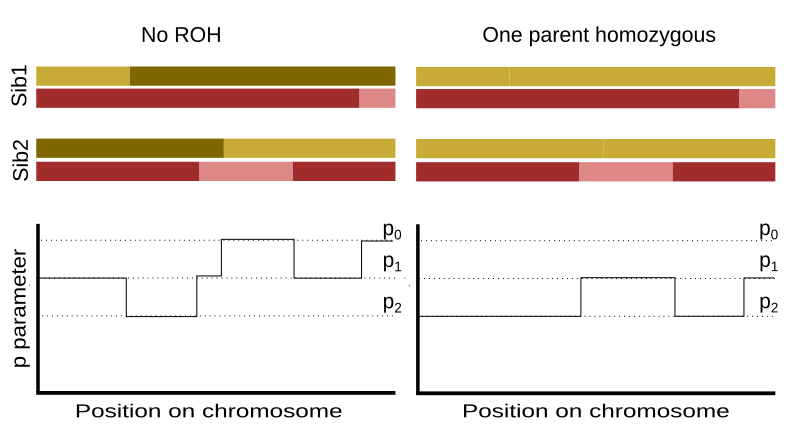
\includegraphics[width=18cm]{plots/inkscape_finalImg/schematic_sib.png}
    \centering
    \caption{IBD sharing between siblings without and with ROH. In top row, recombined chromosomes inherited from parents by a pair of siblings are shown. On the left, the parents have unrelated chromosomes, and on the right one parent has a homozygous pair of chromosomes. The bottom row shows the expected proportion of differences (p) along the chromosome in both the cases. p can take values of $p_0$, $p_1$ or $p_2$ which are expected proportion of differences in IBD states 0,1 and 2 respectively.  }
    \label{fig0:schematic}
\end{figure}


There are numerous methods that utilize population allele frequencies, phase information, recombination maps, or genotype calls to estimate the relatedness coefficient \cite{huff_maximum-likelihood_2011,li_relationship_2014,li_accurate_2014,thornton_estimating_2012}. PLINK, a popular tool to infer relatedness coefficient in diploid genotype data, estimates IBD probabilities from observed IBS, using the allele frequencies at each Single Nucleotide Polymorphism (SNP) in the analyzed samples \cite{purcell_plink_2007}. KING is another widely used software that allows relatedness inference with genotype data in homogeneous populations using population allele frequencies in the samples (KING homo), but can also work with structured populations with no good population allele frequencies using heterozygosity estimates from each sample (KING robust) \cite{manichaikul_robust_2010}. . 

\begin{table}
\caption{\label{tab:Table 1}IBD sharing probabilities for different relations}
\begin{tabular}{|c|c|c|c|}
    \hline
    Relatedness & $k_0$ & $k_1$ & $k_2$\\
    \hline
    Unrelated & 1 & 0 & 0\\
    \hline
    3rd Degree & 0.75 & 0.25 & 0\\
    \hline
    2nd Degree & 0.5 & 0.5 & 0\\
    \hline
    Siblings & 0.25 & 0.5 & 0.25\\
    \hline
    Parent-Child & 0 & 1 & 0\\
    \hline
    Identical/twins & 0 & 0 & 1\\
    \hline
\end{tabular}
\label{table1}
\end{table}

\subsection{Problems with ancient data, and methods that address these issues}
One major issue with applying the above mentioned methods to ancient DNA is that, frequently, the amount of endogenous DNA is very low, making it very difficult to get genotype calls.
Several methods surmount this problem by using genotype likelihoods \cite{lipatov_maximum_2015,korneliussen_ngsrelate_2015}.In this way, it is possible to account for the uncertainty in genotype calls by summing over all possible genotypes weighted by their genotype likelihoods. However, these approaches typically still require at least 2x coverage, since genotype likelihoods may not be very informative at lower coverages. Apart from the low amount of endogenous DNA sequences present, ancient DNA analyses often have additional challenges like contamination from present-day DNA \cite{peyregne_authentict_2020}, absence of a good reference panel, and ascertainment bias in case of captured sequences. In cases where the allele frequency or a reference panel for the target population is not available, it is possible to use allele frequency from a modern population from the same geographic location, or to try using population allele frequencies from multiple potentially close populations. However, incorrect assumptions may cause the individuals in the target population to look more similar or different to each other \cite{amorim_understanding_2018}. Several methods have been proposed to estimate relatedness without a reference panel, but many of these require either $>4x$ coverage \cite{waples_allele_2019}, or a large sample size to get an estimate of population allele frequencies from the samples \cite{theunert_joint_2017}. In this study, we show that contamination can cause some of the individuals in ancient populations to look more unrelated than they are. This happens because of comparison of endogenous reads to contaminating reads which yields more differences than comparison of endogenous reads from the ancient individuals. It is worth mentioning that different DNA libraries may have different levels of contamination, even when they have been sampled from the same specimen. Hence, contamination can reduce the power to detect related pairs, especially when the target population is quite diverged from contaminating population(s). In addition, the genomes of target individuals may have long runs of homozygosity (ROH) due to a small population size, or recent inbreeding. Long ROH causes related individuals to seem genetically closer to each other, while does not affect the genetic distance between unrelated individuals. This effect may cause an increase in false positives. Moreover, ancient DNA is commonly captured with a SNP array to enrich for endogenous sequences. The way that these SNPs are defined (e.g. selecting SNPs variable in certain individuals) becomes relevant, because relatedness methods based on the fraction of sites in different IBS states are highly sensitive to ascertainment bias. KING robust, for example, differentiates between different relatedness by plotting KING‐robust KINship against fraction of sites in IBS0 \cite{manichaikul_robust_2010}. Another method from Rosenberg,2006 \cite{rosenberg_standardized_2006} uses the fraction of sites in all three IBS states to classify related individuals in the HGDP-CEPH Human Genome Diversity Cell Line Panel. These methods may give different results when applied to data with different ascertainment schemes \cite{waples_allele_2019}. 

Several limitations with ancient DNA mentioned above, such as low coverage, the absence of population allele frequencies or a reference panel, and ascertainment bias are resolved by a software called READ. This software addresses the problem of unavailability of genotype calls by randomly sampling alleles from each individual. A string of these alleles at each position (called pseudo-haploids) are then compared to other individuals to calculate average pairwise genetic distances, which in turn are used to infer relatedness. The limitations are that the software can identify only up to second degree relatives, without differentiating between siblings and parent-child, which may be crucial when making pedigrees.

\subsection{How our method works}
Here, we present KIN (Kinship INference), a Hidden Markov Model (HMM) to estimate relatedness and IBD from low-coverage ancient DNA data. KIN can detect up to \nth{3} degree relatives, and differentiates between siblings and parent-child. KIN is also able to take into account ROH, contamination and ascertainment bias. We validate the performance of KIN using simulations and show that we are able to infer relatedness in real data from two datasets: a group of Neandertals and a group of Bronze age individuals.


\section{Methods}

The core of  KIN is a HMM that aims to infer relatedness and IBD sharing between a pair of low-coverage individuals, optionally taking ROH tracts and contamination estimates in each individual into account. If the locations of ROH tracts are unknown, we provide another HMM to coarsely estimate the location of ROH for samples  of sufficient coverage ($\geq 0.5x$). Our method is available on \url{https://github.com/DivyaratanPopli/KIN_snakemake} along with a \textt{snakemake} \cite{koster_snakemakescalable_2012} pipeline to generate the input files for the models directly from bam files. 


\subsection{Relatedness Model overview} 
Our relatedness model assumes we have low-coverage genome sequences for a number of individuals from the same population, and our goal is to infer which pairs of individuals are related. We subdivide the genome into $L$ large windows (typically of size 10Mb). The inputs of our algorithm are i) the number of overlapping sites for the $w$-th window $N_w$ for which both samples have at least one read available, ii) the expected number of pairwise differences $D_w$ at these sites, and iii) the probability of ROH in windows, by default obtained from ROH-HMM described in a following section. $D_w$ is the number of sites that are different between a pair of individuals, and can be estimated accurately for high coverage data by comparing genotypes. For low coverage samples, $D_w$ is typically calculated by comparing randomly-sampled reads (or pseudo-haploid sequences) \cite{haak_massive_2015}. However, such an approach may result in loss of data, and hence we calculate $D_w$ by implicitly summing over all possible samplings:
\begin{align}\label{eq:x}
D_w &= \sum_s \nu_i(s) (1-\nu_j(s)) + (1-\nu_i(s)) \nu_j(s)
\end{align}
Here, $\nu_i(s)$ and $\nu_j(s)$ are the derived allele frequencies for individuals i and j respectively, at SNP index $s$ in a window.
Throughout, we will use bold-face notation to refer to the vector (or matrix) collecting  all the terms, e.g. $\BD = (D_1, D_2, \dots D_L)$. The KIN-HMM uses $\BD$ and $\BN$  to classify each window into three hidden states $Z_w \in$ ($0$, $1$, $2$), reflecting zero, one or two chromosomes shared IBD. Likewise, we classify each window into one of three possible ROH state $H_w \in$ ($0$, $1$, $2$), reflecting, zero, one or both individuals being in a run-of-homozygosity at this genomic location.

There are two additional parameters, $\pi$ and $\mathbf{A}$. The initial probabilities $\pi$ give the probabilities of being in each state $Z$ at the beginning of each chromosome, which we set to uniform for simplicity. The transition matrix $\mathbf{A}$ gives the probability of moving from state $i$ to state $j$, given by $a_{ij}$, and is fixed for each relatedness category (see section YYY). For compactness of notation, we group the fixed parameters: $\theta = (\BN, \mathbf{A}, \pi)$. 

We compute the complete data likelihood for the HMM:

\begin{align}\label{eq:1}
\log P(\BD,\BZ|\BH, \theta) &= \log P(\BD|\BZ,\BH, \theta) + \log P(\BZ |\theta) \nonumber\\
&= \sum_w \log P(D_w|Z_w,H_w, \theta) + \sum_w \log P(Z_w |Z_{w-1},\theta) + \log P(Z_0|\theta)
\end{align}

\subsubsection{Emission probability}
Using this set up, we can isolate the emissions $P(D_w | Z_w, H_w ,\theta)$ from equation \ref{eq:1} and optimize them alone. The number of shared sites $N_w$ is the only parameter in $\theta$ that affects the emissions. 

Assuming sites are equally distributed and independent would result in the binomial likelihood:
$$P(D_w|Z_w, H_w, N_w) \sim \text{Binom}[D_w ; p(Z_w, H_w), N_w] \text{,}$$

where, $p$ is the expected proportion of differences we would expect for a particular IBD and ROH state. If the two individuals are unrelated in a particular window (i.e. $Z_w = 0$), then the expected proportion of pairwise differences depends solely on the effective population size, and we denote this proportion with $p_0$. Note that $p_0$ does not depend on the presence of ROH, since this does not change expected proportion of differences between unrelated individuals. If the two individuals share one or even both copies of the genome IBD, we would expect the proportion of differences to be reduced to $p_1 = \frac{3}{4} p_0$, and $p_2 = \frac{1}2 p_0$, respectively, since either one or two of the four possible comparisons will be between identical chromosomes \cite{kuhn_estimating_2018}. Thus, $p(Z_w=i, H_w=0) = p_i$.

The proportion of differences between unrelated individuals $p_0$ is an important parameter. We follow READ \cite{kuhn_estimating_2018} and estimate it as the median of differences for all possible pairs of individuals, which should work well if the majority of individuals in the samples are unrelated. We set $p_1$ to $(3/4)p_0$ and $p_2$ to $p_0/2$. 

The presence of inbreeding adds an additional complication, as it is possible that all chromosomes are shared between individuals, so that the expected differences should be zero. An example would be inbred regions in two bones from the same individual. However, as we do all our calculations in large windows, the start/end positions of windows may not coincide with that of ROH tracts, and we found that setting expected proportion of differences in this case ($p_3$) at $p_2/2$ works well in practice.


Taken together, we can summarize $p$ in the following matrix, where rows give the state of $Z_w$, and columns of $H_w$:
\begin{equation}\label{eq:2}
    p(Z_w, H_w) = \left[\begin{array}
{rrr}
p_0 & p_0 & p_0 \\
p_1 & p_2 & p_3 \\
p_2 & p_3 & p_3
\end{array}\right]
\end{equation}


The effect of these considerations is that even though we have nine possible combinations of $Z_w$ and $H_w$ for each window, there are actually only four unique $p$-parameters $p_i$ with $i$ $\in$ (0,1,2,3). 

\paragraph{Beta Binomial Model}
The Binomial Model laid out above assumes that sites are independent. However, due to genetic linkage, nearby sites will be correlated and we find that the data often has considerably higher variance than would be expected from a binomial model. We take this into account by adding an overdispersion parameter $\delta$ that allows for variation in the $p$ between windows. Note that, just like $p(Z_w,H_w)$, $\delta(Z_w,H_w)$ has effectively four unique parameters $\delta_i$ with $i$ $\in$ (0,1,2,3). This is due to the fact that several combinations of $Z_w$ and $H_w$ can lead to comparison between same number of unique chromosomes, and such states will have same mean as well as the same variance. This results in the beta-binomial likelihood, that can be fitted to the data (fig. S\ref{figS1:binom})).  

\begin{align}\label{eq:3}
P(D_{w}|p_i,\delta_i,N_w) &\sim BB[D_w; N_w, p_i, \delta_i] \nonumber\\
&= \binom{N_w}{D_w}\frac{B(D_w+p_x \delta_{i}, N_w-D_w+ \delta_{i}(1-p_{i}))}{ B(p_{i}\delta_{i}, (1-p_{i})\delta_{i})}.
\end{align}

This parameterization of the beta distribution in terms of expected value $p$ and overdispersion $\delta$ is also called the Balding-Nichols-model \cite{balding_method_nodate}, and is distinct from the more common parametrization in terms of $\alpha$ and $\beta$. It is worth mentioning here that $D_w$ is estimated as a sum of probabilities (see section XX), while both $D_w$ and $N_w$ may undergo contamination correction, which causes these estimates to be non-integral. We calculate factorials required in Beta Binomial likelihood with Gamma function, which is continuous and hence does not require integral values.   

\subsubsection{Estimation}


Emission probabilities are estimated with Expectation-Maximization (EM) algorithm. In each iteration of the algorithm, the Expectation step involves forward-backward algorithm to calculate $P(D, Z| H, \theta, \delta)$. 



In maximization step we use these joint probabilities to optimize $\delta_i$ for each state i $\in$ (0,1,2,3), and update emission probabilities. Iterations are run, until the complete data log likelihood stops changing. 

\paragraph{Initialization}
The value of $\delta_i$ is unknown to start with, and is set to a random value.

\paragraph{Expectation step}
In the $t$-th iteration, we calculate the posterior probability of each IBD state in each window $\gamma^{(t)}_{wi} = P(Z_w=i | \BD, \BH, \theta, \delta^{(t)})$ using the forward-backward algorithm, where $\delta^{(t)}$ is the current guess for delta.

\paragraph{Maximization step}
The only free parameters we estimate in the M-step are the overdispersion parameters $\delta_i$. We do this optimization using a cost function, which is the log-emission probability weighted by the posterior probabilities of the hidden states $\gamma_{wi}$ and the ROH state-probabilities $h_{w\omega}$.


\begin{align}\label{eq:4}
\mathcal{C} &= \mathbb{E}[\log P(D_w|Z_w, H_w, \theta, \delta^{(t-1)}]\nonumber\\
&= \sum_{w=1}^L \sum_{i=0}^2\sum^2_{\omega=0} \log P(D_{w}|Z_w, H_w, N_w, \delta^{(t-1)}, p)h_{w\omega}\gamma_{wi}
\end{align}


Using equation \ref{eq:2}, we simplify this by grouping all the terms that would result in the same $p$, i.e.

\begin{align*}\label{eq:5}
g_{w0} &= \gamma_{w0}\\
g_{w1} &= \gamma_{w1} h_{w0}\\
g_{w2} &= \gamma_{w2} h_{w0} + \gamma_{w1} h_{w1}\\
g_{w3} &= \gamma_{w2} h_{w1} + \gamma_{w2} h_{w2} + \gamma_{w1} h_{w2}
\end{align*}

So we can rewrite equation \ref{eq:4} as:
\begin{align}\label{eq:6}
\mathcal{C} &= \sum_{w=1}^L\sum_{i=0}^3 \log P(D_{w}|Z_w, H_w, N_w, \delta_i, p_i)g_{wi}
\end{align}

Since each term in equation \ref{eq:6}  depends on only one $\delta_i$ and not on different IBD and ROH states, we can optimize for them independently.

We realized that different cases of relatedness have different number of IBD states possible. For example, siblings may have all three IBD states present while a Parent-Child has only $Z_w=1$. This may cause some overfitting problem, when we apply a Parent-Child HMM to a dataset corresponding to siblings. We show a simple example of this problem in fig. \ref{figS4:bndsbeta}. We avoid this problem by constraining the parameter space of $\delta$. 
In particular, the variance of a beta distributed random variable $X$ is:
\begin{align}\label{eq:7}
    var(X) = \frac{p(1-p)}{\delta + 1}
\end{align}
We constrain $\delta$ such that  the variance is less than a threshold T:

\begin{equation}\label{eq:8}
    \frac{p(1-p)}{\delta + 1}  < T
\end{equation}

We choose T for each beta distribution such that the distributions do not overlap much.

\subsubsection{Relatedness cases}
We run our model for the following relatedness cases: Unrelated, $5^{th}$ Degree, $4^{th}$ Degree, $3^{th}$ Degree, Grandparent-Grandchild, Avuncular, Half-siblings, Parent-Child, Siblings, Identical.
We estimated the transition matrix corresponding to each relatedness case using simulations (see section XX). While testing KIN on simulations, we found that classification performance for $4^{th}$ and $5^{th}$ degree relatives is poor, and we have low power to distinguish them from unrelated pairs of individuals. However, we would like to classify 4-th and 5-th degree relatives as unrelated, and so we include these cases in the algorithm. Similarly, we observe that we have low power to differentiate between half-siblings, avuncular and grandparent-grandchild, and we merge these classifications as $2^{nd}$ degree in the final results. We report the final pairwise classification in the following categories: Unrelated, Third Degree, Second Degree, Parent-Child, Siblings, Identical individuals. We output the relatedness corresponding to the maximum likelihood model, and the confidence as given by the log likelihood ratio between the two highest likelihood models. The log likelihood-ratio is commonly used in likelihood-ratio tests to compare nested models. However, in our cases, models are not nested, and so standard likelihood-ratio theory does not apply. For this reason, we use the log likelihood ratio between the two best models as a statistic to assess the confidence in our classifications, and use simulations to obtain critical values (Fig \ref{fig3:cutoff}).

Hidden IBD state of each window ($Z_w$) is estimated using standard Viterbi algorithm, and $\BZ$ corresponding to the most likely model are returned. 

\subsubsection{ROH estimation model}
Our HMM to detect ROH tracts works similar to the relatedness model described above, but we only consider one individual at a time, and only positions covered by at least two reads. For each site, we calculate the proportion of reads that carry different alleles, and sum them up in windows along the genome. We call the vector with the number of differences $\mathbf{\Delta}$, and the vector with the number of sites with at least two reads $\mathbf{N}$.   Our model has two possible hidden states: homozygous (state $3$), and non homozygous (state $2$). As above, we collect the hidden states in a vector $\mathbf{Y} = (Y_1, \dots Y_w, \dots, Y_L)$. The complete data likelihood for the model in this case is then:

\begin{align}\label{eq:10}
    log P(\mathbf{\Delta},\mathbf{Y}|\Theta) &= log P(\mathbf{\Delta}|\mathbf{Y},\Theta) + log P(\mathbf{Y}|\Theta)\nonumber\\
 &= [\sum_{w} log P(\Delta_w|Y_w, \Theta) + \sum_{w} log P(Y_w|Y_w-1, \Theta)] + P(Y_0| \Theta)
\end{align}

We give details on the transition, emission and their estimation below.

In this case, transitions are not known, and we estimate both transitions and emissions using an EM algorithm. We calculate the emissions using beta-binomial likelihood, and fix the mean of the distributions at expected proportion of differences in a ROH tract ($p_3$) and expected proportion of differences in a non-ROH tract ($p_2$). The expectation step outputs the posterior probability $\Gamma$ of being in state $Y_w=3$ or the state $Y_w=2$ in each window. The M-step for emissions in analogous to that in the KIN model (eq. \ref{eq:4}):

\begin{align}\label{eq:11}
\mathcal{C} = \sum_{w=1}^L \sum_{i=2}^3 P(\Delta_w|\eta_{i},p_{i}) \Gamma_{wi} ,
\end{align}
where $P(\Delta_w|\eta_{i},p_{i})$ is a beta-binomial probability given by eq. \ref{eq:3}.

While testing this method on low coverage data, we observed that some pair of individuals may have few sites in each window, resulting in the proportion of differences to become close to 0 or 1. This may result in a high variance, and can potentially influence our estimation of $\eta$. To avoid the estimated Beta distributions from flattening to fit this high variance data, we set $Y_w=0$ for windows with high differences (fig. S\ref{figS5:ROHforced}). Finally, to estimate transitions, we initialize the transition matrix with 0.2 for the off-diagonal entries, and update it using the standard Baum-Welch update step \cite{baum_maximization_1970}. 

\subsubsection{Contamination}
Contamination by the DNA from present-day people is a common feature in ancient DNA \cite{peyregne_present-day_2020}. Even low levels of contamination may make samples look less similar, and thus distort relatedness analyses. This issue is particularly pronounced  when analyzing populations with low diversity, where even $<5\%$ contamination can cause loss of power to detect family relations (Skov et al.,2022 (in press)). To address this issue, we develop a heuristic that adjusts both $D_w$ and $N_w$ to remove contamination from the data.

We conceptualize contamination in the following way. If data from individual $i$ has a known contamination rate of $C_i$, this means that any particular read drawn from this individual will actually come from that individual with probability $1-C_i$. With probability $C_i$ the read comes from a contaminant. Thus, when comparing two reads, one drawn from individual $i$ and the other drawn from individual $j$, there are three possible cases: First, with probability $(1-C_i)(1-C_j)$, both reads are endogenous and we can use them to infer relatedness. With probability $C_i(1-C_j) + C_j(1-C_i)$, one read is endogenous and the other is contaminant. Finally, with probability $C_iC_j$, both reads are contaminant. If we make the simplifying assumption that both $C_i$ and $C_j$ are small, the terms of the order of $C^2$ can be ignored. Then, we compare contaminant read to endogenous read with the probability $C_{ij} = C_i + C_j$.

Given that we know the level of contamination (estimated from other methods),our goal then, is to estimate the expected number of differences from comparison of endogenous reads $\mathbb{E}[D_w^{'}]$, and the total number of sites with overlapping endogenous reads $\mathbb{E}[N_w^{'}]$. To estimate $\mathbb{E}[D_w^{'}]$, we first need to calculate $P(c=0|d=1)$. Here, $c$ is a binary variable with value $0$ or $1$ denoting that the comparison at a site is between endogenous reads, or between endogenous and contaminant reads respectively. Similarly $d$ is a binary variable taking values 0 and 1 for seeing no difference, or a difference, when comparing the reads at a given site. We can further expand this probability:

\begin{align}\label{eq:12a}
    P(c=0|d=1) &= \frac{P(d=1|c=0)P(c=0)}{P(d=1)} \nonumber\\
\end{align}

Here, $P(d=1|c=0)$, referred later to as $\rho_{ij}$ for simplicity, is equivalent to the proportion of differences when we compare endogenous reads from individuals $i$ and $j$. This can be estimated by considering that the proportion of pairwise differences $P(d=1) =\frac{\sum_w D_w}{\sum_w N_w}$, referred to as $o_{ij}$ later, can be expressed as a linear combination of the proportion of differences between endogenous reads and that between endogenous and contaminant reads \cite{peyregne_present-day_2020}. 
\begin{align}\label{eq:13}
    o_{i,j} = (1-C_{ij}) \rho_{ij} + C_{ij} \phi \nonumber\\
    or, \rho_{ij} = \frac{o_{ij} - C_{ij} \phi} {1 - C_{ij}}
\end{align}

Here, $\phi$ is the probability of seeing a difference when an endogenous read is compared to a contaminant read, and is equivalent to the average sequence divergence between individuals of the target and contaminating populations.
Given this information, we can rewrite eq. \ref{eq:12a}:
\begin{align}\label{eq:12}
    P(c=0|d=1) &= \frac{(1 - C_{ij}) \rho_{ij}}{(1 - C_{ij}) \rho_{ij} + C_{ij} \phi} \nonumber\\
\end{align}
We can further write $\mathbb{E}[D_w^{'}]$ as $D_w P(c=0|d=1)$:
\begin{align}
    \mathbb{E}[D_w^{'}] &= D_w\frac{(1-C_{ij})\rho_{ij}}{(1-C_{ij}) \rho_{ij} + C_{ij} \phi}\\
\end{align}

Similarly, we derive $\mathbb{E}[S_w^{'}]$ as the estimate for the number of sites that do not show pairwise differences.
\begin{align}
    \mathbb{E}[S_w^{'}] &= (N_w-D_w) P(e=1|d=0) = (N_w - D_w)\frac{(1-\rho_{ij})(1-C_{ij})}{(1-\rho_{ij})(1-C_{ij}) + C_{ij}(1-\phi)}\\
\end{align}

We added $D_w^{'}$ to $S_w^{'}$ to get the corrected number of overlapping sites $N_w^{'}$  

------------------------------------------extra stuff-----------Do not read--------------------------------


If we look at one site in the window, we could find either no difference in reads from individuals $i$ and $j$ ($d_s$=0), or a non-zero difference ($0<d_s<=1$). Here $d_s$ is the probability of seeing a difference at site $s$, and $\sum_{s \in w} d_s =D_w$. We ask, what is the    

If we make the simplifying assumption that both $C_i$ and $C_j$ are small, terms of the order of $C^2$ can be ignored and there are just two cases: with probability $C_{i,j} =C_i + C_j$, one of the reads stems from a contaminant, and we effectively compare a contaminant fragment with an endogenous one. The probability that they differ is the average divergence between target and contaminating population, which we denote with $\phi$. The other case (w. p. $(1-C_{i,j}$) is where we compare two endogenous reads, which will differ with probability

\begin{equation}
    p_{e} = \frac{p_{obs}-\phi C_{i,j}}{1-C_{i,j}}
\end{equation}

Here, $$p_{obs} = \frac{\sum_w D_w}{\sum_w N_w}$$


We estimate $\hat{D_c} = C_{i,j} N_{tot} \phi$ and $\hat{D_e} = (1-C_{i,j}) N_{tot} p_{obs}\phi$.
If there are $N_{obs}$ overlapping sites in a window, $N_{c} = C_{i,j}N_{obs}$ of them will include a contaminant allele, and $N_e = (1-C_{i,j})N_{obs}$ will be between endogenous alleles.

For KIN, we can use $N_e$ as an input (for each window), but we also need the proportion of differences, $D_e$. For this, we use the assumption that the proportion of sites where the contaminant differs from our samples is 

$$\phi = \frac{D_c}{N_c} = \frac{D_c}{C_{i,j} N_{obs}}, $$
and thus $D_c = C_{i,j} \phi N_{obs}$. 

We can think of $p_c$ and $\rho$ as empirical likelihoods that a particular site shows a difference between two reads, given that the comparisons contain only endogenous or one contaminant read, respectively. 
\begin{align}
    P(E|D) &= \frac{P(D|E)P(E)}{P(D)} \nonumber\\
    \mathbb{E}[D_e] &= D_{obs} P(E|D) = D_{obs}\frac{p_e (1-c)}{p_e(1-c) + c\rho}\\
    \mathbb{E}[S_e] &= D_{obs} P(E|\text{not} D) = S_{obs}\frac{(1-p_e)(1-c)}{(1-p_e)(1-c) + c(1-\rho)}
\end{align}

And for calculating $N_{e}$, we added $D_{e}$ to $S_{e}$    

The goal is that given $C_{i,j}, p_e, \BN and \BD$ to calculate adjusted $\hat{\BN}$ and $\hat{\BD}$ that reflect the endogenous proportion only.

, and the observed proportion of differences between individuals $i$ and $j$ as $p_{oij}$. We calculate average endogenous pairwise difference $p_{eij}$ for individuals i and j as follows \cite{noauthor_ancient_nodate}:
\begin{align}
    p_{oij} = C_{ij}  p_c + (1-C_{ij})  p_{eij}\\
    or, p_{eij} = \frac{p_{oij} - C_{ij}  p_c}{1-C_{ij}} 
\end{align}

Given $p_{eij}$, we would ideally like to calculate the complete data log likelihood for the relatedness model while summing over all possible differences we could have in a window weighted by the probability of seeing that difference. 



\paragraph{Short version}
With contamination, we do not observe the number of differences $D_{true}$ and total number of comparisons $N_{true}$ directly, but instead need to approximate them. The window-subscript is omitted in the following for clarity:
\begin{equation}
    P(D_{\text{obs}} | N_\text{obs}, Z, \theta) \approx 
    P( \hat{D} | \hat{N}, Z, \theta)
\end{equation}
We do that by calculating the probability that a single read is endogenous given it has a difference.
\begin{align}
    \hat{D} = \mathbb{E}[D | D_{\text{obs}}, c] &= 
    D_{\text{obs}} P(E_i | D_i=1) \\
    &= D_\text{obs} \frac{P(D_i=1 | E_i)P(E_i)}{P(D_i=1)}\\
    &= D_\text{obs} \frac{(1-c)p_e}{(1-c)p_e + c p_c}
\end{align}

and likewise for reads that do not have a difference
\begin{align}
    \hat{S} = \mathbb{E}[S | S_{\text{obs}}, c] &= 
     S_\text{obs} \frac{(1-c)(1-p_e)}{(1-c)(1-p_e) + c (1-p_c)}
\end{align}

and $\hat{N} = \hat{S} + \hat{D}$

\begin{equation}
    P(D_{\text{obs}} | Z, N_\text{obs}, \theta) = \sum_n\sum_d P(D_{\text{obs}}, N_\text{obs} | D_w=d, N_w, C_i, C_j)\underbrace{P(D_w=d | N_w, Z, \theta)}_\text{old likelihood}
\end{equation}

i.e. we sum over all possible $D_w$, $N_w$. Instead, we use

\begin{align}
    P(D_{cor},Z|D,H,\theta,c,p_c) &= P(D_{cor}|Z,D,H,\theta,c,p_c) P(Z|D,H,\theta,c,p_c)\nonumber\\
    &= [\prod_{w} [\sum_\kappa P(D_{cor,w}|Z_w, H_w, \theta,c,p_c) P(D_{cor,w}=\kappa)] \prod_{w} P(Z_w|Z_{w-1}, \theta)] P(Z_0| \theta)
\end{align}



We realize that this calculation would be time consuming, and would further complicate the HMM. To avoid this, instead of using weighted sum of all possible $\kappa$, we use $E(D_{cor,w}|Z_w, H_w, \theta,c,p_c)$. This simplifies the equation 21 to :

\begin{align}
    P(D_{cor},Z|D,H,\theta,c,p_c) &= P(D_{cor}|Z,D,H,\theta,c,p_c) P(Z|D,H,\theta,c,p_c)\nonumber\\
    &= [\prod_{w} P(E(D_{cor,w})|Z_w, H_w, \theta,c,p_c) \prod_{w} P(Z_w|Z_{w-1}, \theta)] P(Z_0| \theta)
\end{align}

We calculate $E(D_{cor,w})$ as shown:

\begin{align}
    E[N_e] + E[N_c] = N\\
    E[D_e] + E[D_c] = D
\end{align}

Probability of comparing endogenous reads at a site where we see a difference:
$$P(\xi | N = 1,D = 1)=\frac{(1-c) p_e}{c p_c + (1-c) p_e} $$
Probability of comparing endogenous reads at a site where we see no difference:
$$P(\xi | N = 1,D = 0)=\frac{(1-c)(1-p_e)}{c (1-p_c) + (1-c) (1-p_e)} $$
Expectation of number of endogenous comparisons in a window:
\begin{align}
    E[\xi | N, D] = D E[\xi | N=1, D=1] + (N-D) E[\xi | N=1, D=0]\\
    = D P(\xi | N=1, D=1) + (N-D) P(\xi | N=1, D=0)
\end{align}



Total number of endogenous sites showing a difference in a window: 
$$D_{cor,w} = D_w* \frac{p_e(1-c)}{p_e(1-c) + c p_c} $$
Total number of endogenous sites showing 0 difference in a window: 
$$S_{cor,w} = S_w* \frac{(1-p_e)(1-c)}{(1-p_e)(1-c) + c (1-p_c)} $$
Total number of endogenous sites in a window:
$$N_{cor,w} = D_{cor,w} + S_{cor,w}$$

This model outputs the contamination-corrected number of differences and overlapping sites in each window.

\subsection{Simulations}

We use simulations both for estimating the transition matrices for all relatedness cases, and for testing and validating our algorithm. All simulations are performed by simulating unrelated individuals using \textt{msprime} \cite{kelleher_efficient_2016}, followed by an additional step where we simulate related individuals using a predetermined pedigree (Figure S\ref{figS10:pedigree}).

\paragraph{Simulations for estimation of transition matrix}

For our simulations of background diversity, we form a population (Pop1) with constant effective size of 10,000 and sample eight diploid individuals (each made up of two haploid individuals) from 2500 generations ago  (fig. \ref{figS10:pedigree}). For each individual, we simulate 22 chromosomes with length $L=100$ Mb and a recombination rate of $r=10^{-8}$ per base pair per generation. We introduce mutations using an infinite sites model with rate  $\mu= 10^{-8}$ per base pair per generation. 

For the pedigree simulations, we first simulate a recombined set of chromosomes for either parent, and combine them to create the progeny. We simulate recombination by first drawing the number of breakpoints as a  Poisson random variable with parameter $rL$, and use a uniform distribution on $[1, L]$ to sample the positions of recombination points. 

\paragraph{Estimating transition matrices}
KIN requires a transition matrix for each relatedness case. For the simplest cases like grandparent-grandchild and siblings, it is possible to calculate the transition matrix from first principles, but for most cases this is difficult  because the relatedness cases include multiple cases, or they are non-Markovian, and so for these cases we obtain transition matrices from our simulations.

For each relatedness case, we estimate the transition matrix  by counting the transition between IBD states for all pairs of individuals at that relatedness level in a training set of XX simulations.

Apart from the related and unrelated individuals in Pop1, we simulated more haploids in three other populations to create scenarios with ascertainment bias and contamination (fig. \ref{figS10:pedigree}). We simulated two haploids to form an individual each from two other populations (Pop2, Pop3) with split time of 3500 and 4500 generations with Pop1, and sampling time of 4000 generations and 2000 generations ago respectively. We identified the sites that were polymorphic among these two individuals, and used these sites to ascertain the genomes of individuals from Pop1. We test out the performance of our method in presence of long ROH ($\sim17\%$), by simulating regions of homozygosity with a Markov chain using transition matrix shown below: 

$$\mathbf{A} = \left[\begin{array}
{rr}
1-10/L & 10/L \\
2/L & 1-2/L  \\
\end{array}\right]
$$

From the steps described above, we got genotypes of 17 individuals in Pop1 in presence/absence of ROH and ascertainment. We further simulated 10 haploids (5 diploid individuals) from Pop4 with split time of 20,000 generations with pop1, sampled from the present time. We calculated the allele frequency for Pop4 at each site, and used it to introduce contamination (with fixed contamination percentage for each individual ($<5\%$) in samples from Pop1. We generated reads (derived/ancestral) for different genomic coverages ranging from 4x to 0.03x at each position for each individual. We specifically generated reads for four different cases: Ancestral-Endogenous, Ancestral-Contaminant, Derived-Endogenous, Derived-Contaminant. The number of reads for each case was sampled from a Poisson distribution with $\lambda$ calculated from the coverage $\zeta$, allele frequency or genotype (G $\in$ 0,0.5,1), and contamination estimate:

\begin{align}
    \lambda_{DE} = \zeta (1-c) G\nonumber\\
    \lambda_{AE} = \zeta (1-c) (1-G)\nonumber\\
    \lambda_{DC} = \zeta c \upsilon\nonumber\\
    \lambda_{AC} = \zeta c (1-\upsilon)
\end{align}

We run simulations with different cases referred to as control (with no ROH, contamination or ascertainment bias), R (with ROH), A (with ascertainment bias), and C (with fixed levels of contamination for each individual). 


\section{Results}


\paragraph{Motivating Example}
We predict different categories of relatedness with KIN, and test it's performance on simulated pedigrees. We use these simulations to find the limits of KIN as well as ROH HMM. We introduce cases of contamination, ascertainment, ROH, and low coverages to compare our method to READ. Finally we apply KIN to published data and show that it can give reliable information about genetic kinship, that may not be available from other available methods. Here, in Fig.\ref{fig1:ibd} we show the output of different Relatedness HMMs when they are applied to a pair of siblings.

\begin{figure}[h!]
    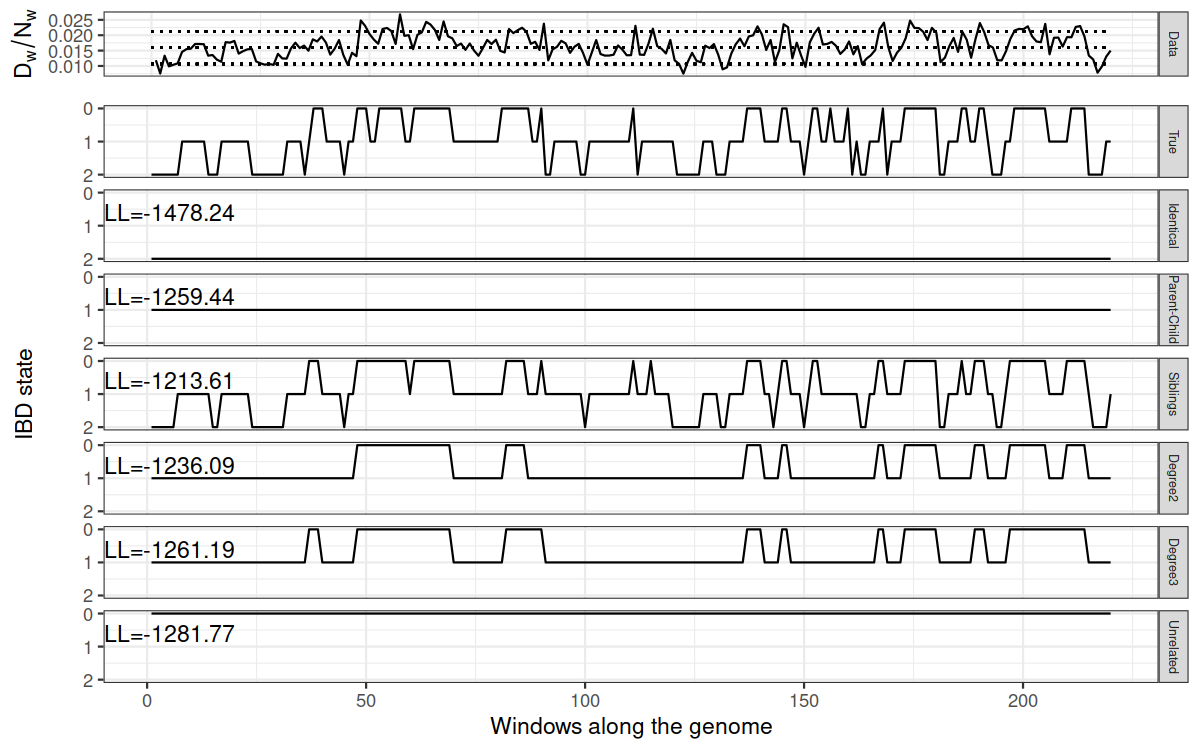
\includegraphics[width=16cm]{plots/plotimg/IBDplot.png}
    \centering
    \caption{\textbf{Comparison of pairwise difference data  and inferred IBD fragments}:  The top panel shows the proportion of differences in each window along the genome for a pair of simulated siblings. Dashed lines represent $p_0$, $p_1$ and $p_2$ estimates. The second panel shows the true IBD state for each window. The remaining panels show the IBD states predicted by particular relatedness models. The log likelihood value for each model is shown on upper left corner of the panel. Light and shaded background represent distinct chromosomes.}
    \label{fig1:ibd}
\end{figure}

We see that in this case, the siblings model predictions match true IBD states the most, as reflected by the highest log-likelihood, and the close match between the estimated and true IBD states. 


\paragraph{Critical Values}
 We plotted the true positive and false positive rates with a cutoff on the log likelihood ratio in Fig.\ref{fig3:cutoff}. Here, and in Fig.\ref{fig4:Comparison_READ_KIN}, we have two relatedness labels: 'Unrelated' and 'Unrelated w/o 3rd Degree'. Unrelated label here refers to KIN performance results when all Unrelated, Fifth Degree, Fourth Degree, Third Degree pairs are labelled as Unrelated. This is useful for comparison to READ, since READ classifies relatedness up to Second Degree. 'Unrelated w/o $3^{rd}$ Degree' refers to the performance results when $3^{rd}$ Degree is classified separately from the unrelated individuals. Fig.\ref{fig3:cutoff} shows that for all relatedness cases except for $3^{rd}$ Degree, the false positive rate is below $5\%$ even when no cut off is used. We observe that for $3^{rd}$ Degree relation, using a cutoff of 1 brings down the false positive rate close to $5\%$ for all coverages except 0.05x. In conclusion, it is recommended to use a cutoff of 1 for most cases.

\begin{figure}[h!]
    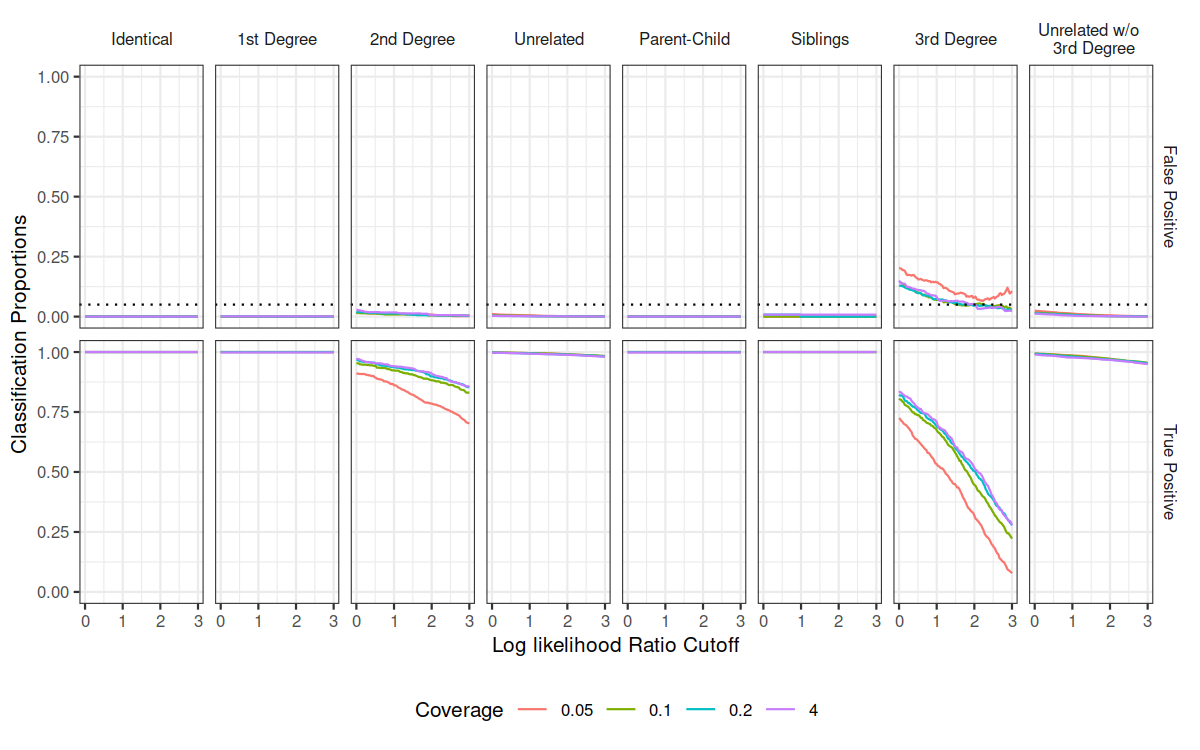
\includegraphics[width=16cm]{plots/plotimg/contam0_inbred0_model_performance_allroc_asc0_plot.png}
    \centering
    \caption{False positive and True Positive rates as a function of cutoff on log likelihood ratio. In top panel, dotted line represents $5\%$}.
    \label{fig3:cutoff}
\end{figure}

In our assessment of critical value for log likelihood ratio, we used the control simulations. However, we test performance of KIN on different simulation cases including case R, which is also based on performance of ROH HMM.

\paragraph{Evaluating the ROH detection}
 Fig.\ref{fig2:ROH} shows the performance of ROH-HMM under cases of control, R, A, C and simulations (described in section Simulations), and for different coverages. We observe that as coverage decreases, the raw heterozygosity estimates become more noisy. In the control case (Fig \ref{fig2:ROH}, we correctly infer that there is no ROH for most of the time, but occasionally we erroneously call some ROH as shown in the figure. We observe that the model predicts ROH probabilities with biases of upto -0.007, -0.081, -0.083, and -0.091 and variances upto 0.006, 0.036, 0.036, and 0.037 in control, R, C, and A cases respectively as shown in supplementary table \ref{tab:Table 2}. The negative bias in all cases shows that on an average, the model over-estimates probability of ROH, and this effect is seen more often at higer coverages. We do not see any large adverse effects of ascertainment bias and contamination on the performance of ROH HMM.


\begin{figure}[h!]
    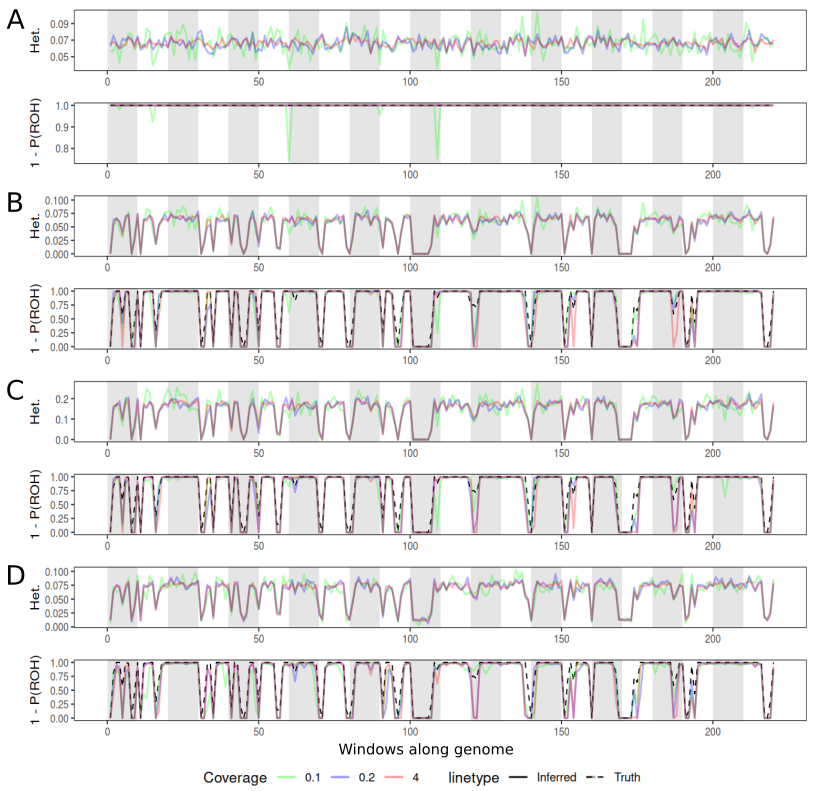
\includegraphics[width=16cm]{plots/inkscape_finalImg/ROHplot_final.png}
    \centering
    \caption{Estimation of ROH probabilities along the genome in simulations with different cases of ROH, contamination, and ascertainment. Top panel shows proportion of differences in a simulated individual along the genome, and the bottom panel shows probability of seeing no ROH. (A) Simulation with no ascertainment, contamination, or ROH. (B) Simulation with ROH. (C) Simulation with ROH and ascertainment. (D) Simulation with ROH and contamination.}
    \label{fig2:ROH}
\end{figure}
We use a cutoff of 1 to compare our method performance to READ, while using a cutoff of 1 standard deviation for READ. Fig.\ref{fig4:Comparison_READ_KIN} shows this comparison using false positive and true positive rates for both the methods at different coverages under different simulations. We show that both methods have similar performance in the control case, and cases with ROH and ascertainment, except for $2^{nd}$ Degree relation, where KIN has higher power, especially at low coverages. We show that adding contamination adversely affects both the False Positve and True Positive rates corresponding to 1st and 2nd Degree relations for READ, while this has no effect on KIN performance.

\begin{figure}[h!]
    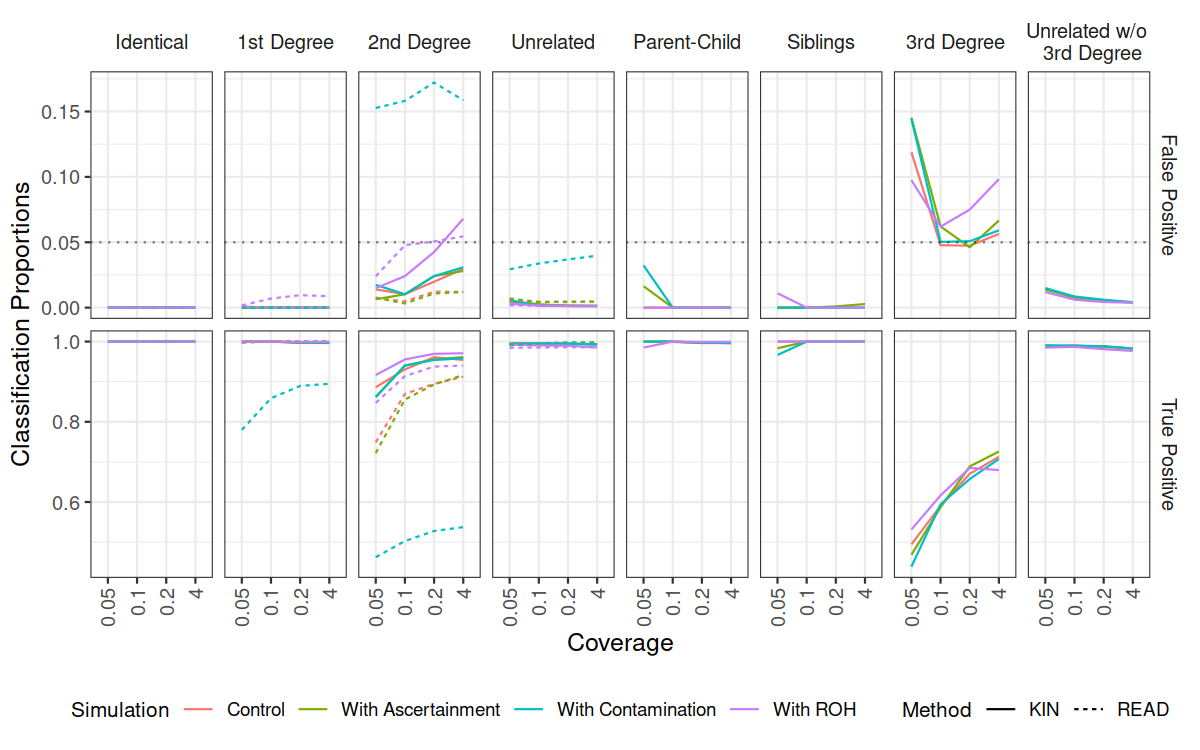
\includegraphics[width=16cm]{plots/plotimg/comparison_plot.png}
    \centering
    \caption{Comparison of KIN with READ using simulations with different coverages, and different cases of ascertainment, contamination and ROH}
    \label{fig4:Comparison_READ_KIN}
\end{figure}


To test KIN on real ancient dataset, we applied it to Neandertal specimens from Chagyrskaya cave in Siberia, Russia. This dataset comprised of 14 specimens that came from neighbouring layers, and hence could possibly belong to contemporary Neandertals who occupied the cave 63 ± 4 to 48 ± 3 kya \cite{kolobova_archaeological_2020-1}. These specimens showed low coverage of nuclear genome (ranging from 0.01x to 12.34x), with 8 samples out of 14 showing $<1x$ coverage. Some of these specimens showed signs of long ROH, and contamination from modern humans as well as Hyena. All these samples were captured with an array targeting for variable sites in high coverage Neandertal and Denisovan genomes and common variations in Africans (Laurits et al.,2022), and we further ascertained this data to variable sites in high coverage Neandertal genomes: Altai Neandertal (Denisova 5) \cite{prufer_complete_2014} and Vindija 33.19 \cite{prufer_high-coverage_2017}. This dataset had all the issues that KIN deals with, and hence we decided to apply it here to see if we could find family relationships that would not be possible with other available methods. Our results for pairwise relatedness for these individuals is shown in Fig.\ref{fig5:Chagyrskaya_KIN}. We found Identical individuals (Chagyrskaya13-Chagyrskaya19-Chagyrskaya1141), $1^{st}$ Degree relative (Chagyrskaya07-Chagyrskaya17), and a $2^{nd}$ Degree relative (Chagyrskaya01-Chagyrskaya60). These results agree with READ (fig. S\ref{figS2:Chagyrskaya_READ}). Both the methods classified Chagyrskaya06-Chagyrskaya14 to be $1^{st}$ Degree relatives with low confidence (table S1), but have been classified as Identical pair in the original study, since Chagyrskaya06 is a tooth sample that fits in mandible which is Chagyrskaya14. We believe that the contradiction is due to non human contamination present in these libraries ($1\%$ and $2.9\%$ respectively). Interestingly, for the pair of Chagyrskaya07-Chagyrskaya17, READ shows that they are first degree relatives, and KIN further identifies them as parent-child. Our result matches with the conclusions of the authors based on additional information from mtDNA. Further, we find a possible $3^{rd}$ degree relative (Chagyrskaya07-Chagyrskaya60). We compared our IBD estimates to lcMLKIN for all pairs for whom READ results (with s.d. >1) and KIN results ($\Lambda$>1) match (fig. S\ref{figS6:Chagyrskaya_ibd}). Chagyrskaya06-Chagyrskaya14 is removed from the analysis. We find that lcMLKIN does create four different clusters for different relatedness. However, the clusters are quite deviated from the expected values, which makes it difficult to identify the relatedness. Identical individuals, for example, are expected to be at $k_0 = 0$ and $r = 1$, and Parent-Child at $k_0 = 0$ and $r = 0.5$. These deviations can be due to ascertainment, contamination, ROH as well as low coverage of samples.



\begin{figure}[h!]
    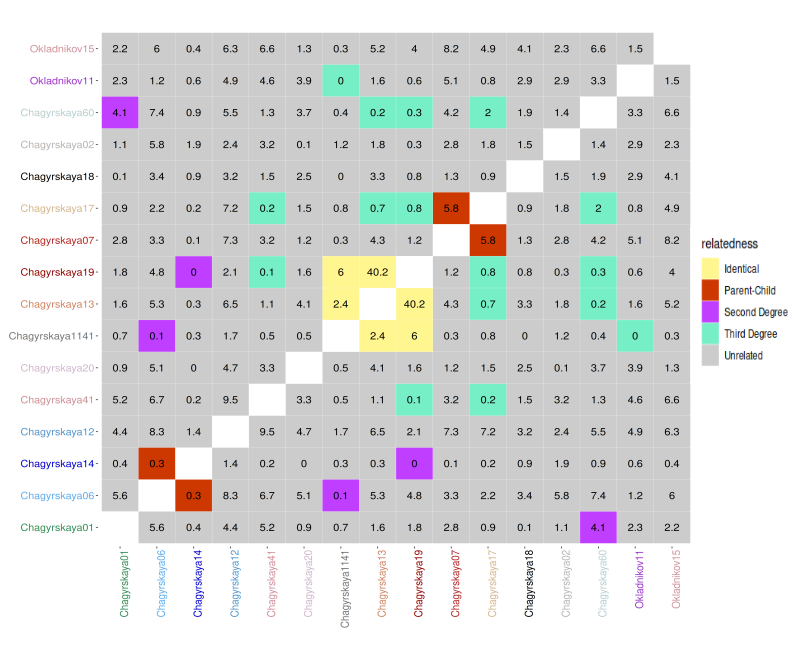
\includegraphics[width=18cm]{plots/inkscape_finalImg/kinplot.png}
    \centering
    \caption{Application of KIN on Neandertal specimens from Chagyrskaya. The color of a square represents the relatedness, while the number within denotes log likelihood ratio between the two maximum likelihood models.}
    \label{fig5:Chagyrskaya_KIN}
\end{figure}

We further applied KIN to a genome-wide dataset of 118 ancient individuals sequenced and analyzed by Mittnik et al.,2019. We compared our relatedness estimates to those obtained from the authors using READ and lcMLKIN, and found that in most cases the three methods agree. Out of 6903 pairs, 346 pairs show different relatedness for KIN and READ (table S2). However, there are only 31 pairs where KIN has $\Lambda >1$. We looked in detail at these pairs, and we found that it is possible to deduce the correct relatedness for several of these pairs by plotting the proportion of differences along the genome. In all the pairs that we analyzed in this way, KIN seems to predict the true relatedness. We show few examples of such cases in fig. S\ref{figS8:eg1}. We found 20 pairs in this subset of 346 pairs where lcMLKIN has sufficient data (Overlapping SNPs $>$ 10000). Among these 20 pairs, we found that lcMLKIN matches KIN estimate in all cases except for pair POST131-POST28 (READ predicts unrelated individuals, lcMLKIN predicts 3rd-5th degree, KIN predicts second degree) and pair AITI72-AITI77A (READ and lcMLKIN predict unrelated, while KIN estimates 3rd degree with log likelihood=1.7).  
We found 43 pairs for which READ estimates first degree, and compared the estimates of lcMLKIN and KIN for these cases (suppl table3). There were a total of 20 pairs where lcMLKIN had sufficient data, and 26 pairs where $loglikelihood ratio>2$ for KIN. Among the 19 overlapping pairs, we found four pairs where KIN and lcMLKIN differ, and a visual inspection shows that in these cases, KIN seems to have the correct estimate (fig. S\ref{figS9:eg2}).  




\section{Discussion}

Several methods are available to estimate relatedness from modern as well as ancient DNA data. We developed a new method to estimate genetic KINship from low coverage data. We show that it is possible to accurately infer relatedness, along with IBD tracts, from such data in presence of long ROH, contamination, as well as ascertainment bias. Our method utilizes Hidden Markov Models to estimate IBD tracts, conditional on a particular relatedness, and we use log likelihoods of these HMMs to find the best fit. This approach of using Hidden Markov Model makes use of the fact that DNA is inherited in blocks, and hence the IBD state in a given window is dependent on the IBD state in the previous window. We use this approach to identify the following pairwise relations: Identical individuals, Parent-Child, Siblings, Second degree, Third degree, Unrelated individuals. We have developed a similar Hidden Markov Model to infer long ROH, and we use the posterior ROH probabilities to make better relatedness inferences. We further use a simple model to correct the pairwise differences in genomic windows in the presence of contamination. 

We used simulated data to validate KIN's performance. We compared KIN's model performance to a widely used software READ to show that our approach gives similar predictions as READ on ideal data with 4x coverage, and without long ROH, ascertainment and contamination, while additionally distinguishing between parent-child and siblings, and identifying third degree relatives. We demonstrate that at low coverage (0.1x) we have higher power to detect first degree relatives compared to READ with similar false positives, while a higher power to identify second degree relatives at the cost of slightly higher false positive rate.
Counter-intuitively, we see that adding long ROH ($~17\%$) to simulations improves the performance of both KIN and READ. READ's performance improves because ROH does not cause any change in pairwise differences between unrelated individuals, while decreasing pairwise differences between related individuals. The higher the relatedness, the higher is the decrease in pairwise differences in presence of ROH. And so, ROH causes higher power for READ which otherwise is a conservative method. KIN performs well for the same reasons, but can additionally differentiate between different combinations of IBD and ROH in genomic windows. Contamination, on the other hand, can affect the performance of READ adversely depending on the amount of exogenous DNA, and the number of individuals contaminated. We show that even at contamination levels  $<=3\%$, and contamination in only 8 out of 17 individuals, READ performance falls. Contamination in more individuals causes a shift in median difference in the population and may cause non contaminated individuals to look more related, thus increasing the false positive rates. On the other hand, an increase in the amount of contamination in a few individuals can make them look more unrelated. KIN, with the implementation of a model to correct for contamination, performs well in this case. Ascertainment causes a decrease in power for both the methods, since it reduces the amount of data. However, the decrease in power is more for READ compared to KIN.

DNA data from Bronze age, Lech valley has low contamination, and no ROH. We demonstrate that KIN matches the results from READ and lcMLKIN for pairs with good amount of overlaps, while adds more information for low coverage samples. As expected from the simulations, KIN is helpful in differentiating between parent-child from siblings, and identifying second and third degree individuals in cases where there is an overlap of only few thousand sites or less, and the other methods are not informative. We show that when applied to Neandertal specimens from Chagyrskaya cave, READ and KIN agree in relatedness estimates for all pairs where both methods have sufficient data. KIN additionally identifies a pair of first degree relatives as parent-child, which is in agreement with mtDNA analysis from the authors. In addition, KIN identifies a third degree relative. We compare IBD estimates from KIN to lcMLKIN and show that KIN's IBD estimates are much closer to the expected estimates, given the relatedness between individuals that has been estimated with both READ and KIN. 
The output of KIN is a table which shows for each pair, the most likely model, and the second best guess, along with a confidence level represented by the log likelihood ratio. Due to the tabular output, KIN is easy to automatise and apply to large datasets. 
One limitation of our approach is that it assumes a single population. In case of population structure, where the sub-populations have very different diversity, KIN may show inaccurate inferences. Our method makes another assumption, that the dataset comprises of at least some unrelated individuals. We estimate $p_0$ as the median of all pairwise differences, and if more than half of the pairs are related to each other, $p_0$ estimate would be biased, and may affect the relatedness inference. In this study, we identify six different cases of relatedness, but in theory our approach can be extended to identify many more such cases, such as double first cousins, using a corresponding IBD state transition matrix.


\section{Supplementary Information}


\begin{table}
\caption{\label{tab:Table 2}Model performance for ROH prediction}
\begin{tabular}{|c|c|c|c|c|c|c|c|c|}
    \hline
    Coverage & Control(bias) & Control(var) & R(bias) & R(var) & RC(bias) & RC(var) & RA(bias) & RA(var)\\
    \hline
    4x & -0.007 & 0.006 & -0.081 & 0.036 & -0.083 & 0.036 & -0.091 & 0.037\\
    \hline
    0.2x & -0.003 & 0.003 & -0.068 & 0.03 & -0.068 & 0.026 & -0.076 & 0.029\\
    \hline
    0.1x & -0.003 & 0.002 & -0.049 & 0.021 & -0.05 & 0.021 & -0.057 & 0.022\\
    \hline
\end{tabular}
\label{table1}
\end{table}

\renewcommand{\figurename}{Fig. S}
\begin{figure}[h!]
    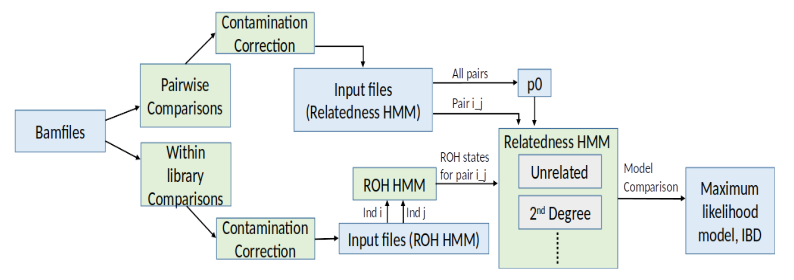
\includegraphics[width=18cm]{plots/inkscape_finalImg/schematic_sup.png}
    \centering
    \caption{Overall schematic of the method. Blue boxes show the data files, while green boxes represent scripts.}
    \label{figS0:schematic}
\end{figure}




\begin{figure}[h!]
    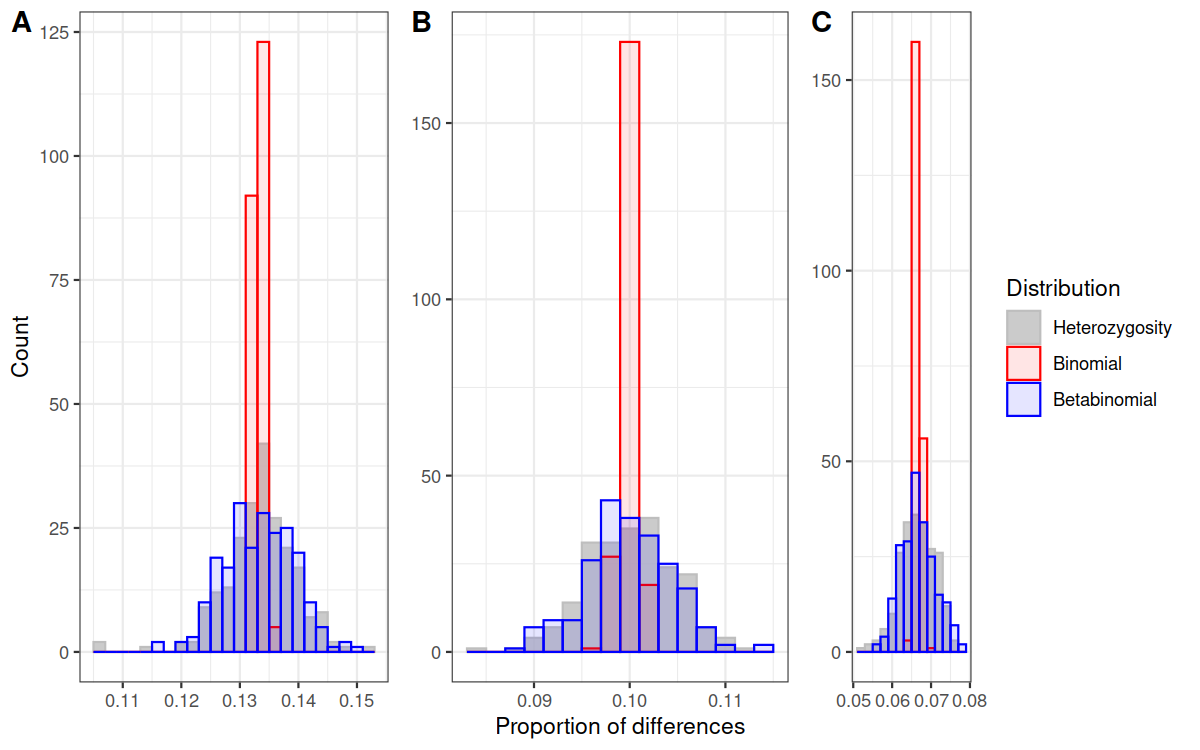
\includegraphics[width=18cm]{supplementary_info/plots/binom.png}
    \centering
    \caption{Comparison of fit with Beta-binomial and Binomial distributions. Data is represented by the histogram of proportion of differences from all windows of a (A) unrelated, (B) Parent-Child, (C) Identical pair of individuals. Binomial parameter p is calculated from the data, while Beta-binomial parameters are estimated with the relatedness HMM.}
    \label{figS1:binom}
    
\end{figure}


\begin{figure}[h!]
    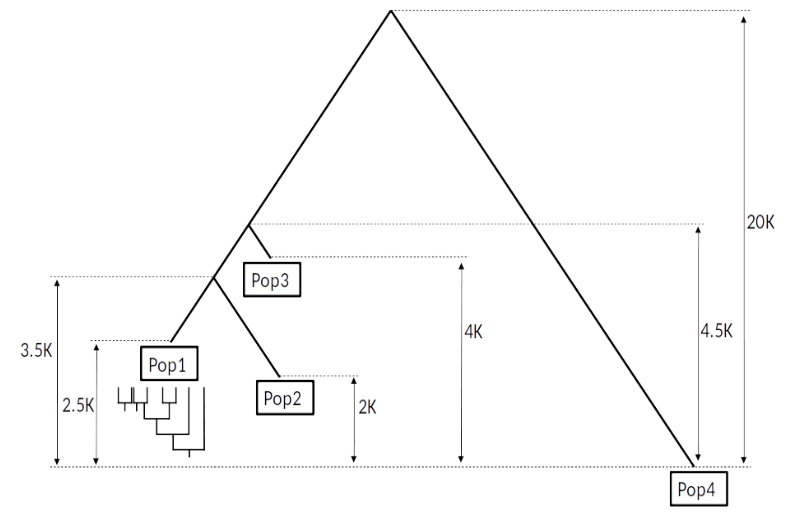
\includegraphics[width=18cm]{plots/inkscape_finalImg/pedigree.png}
    \centering
    \caption{Overview of simulated dataset. We simulated Pop1, and artificially mated unrelated individuals to make a family with upto 5th degree relatives, along with other unrelated and identical individuals (not shown here). Pop2 and Pop3 are simulated so as to introduce ascertainment, while Pop4 is a present day population used to simulate contamination. Split times and sampling times of the populations are shown in generations.}
    \label{figS10:pedigree}
    
\end{figure}


\begin{figure}[h!]
    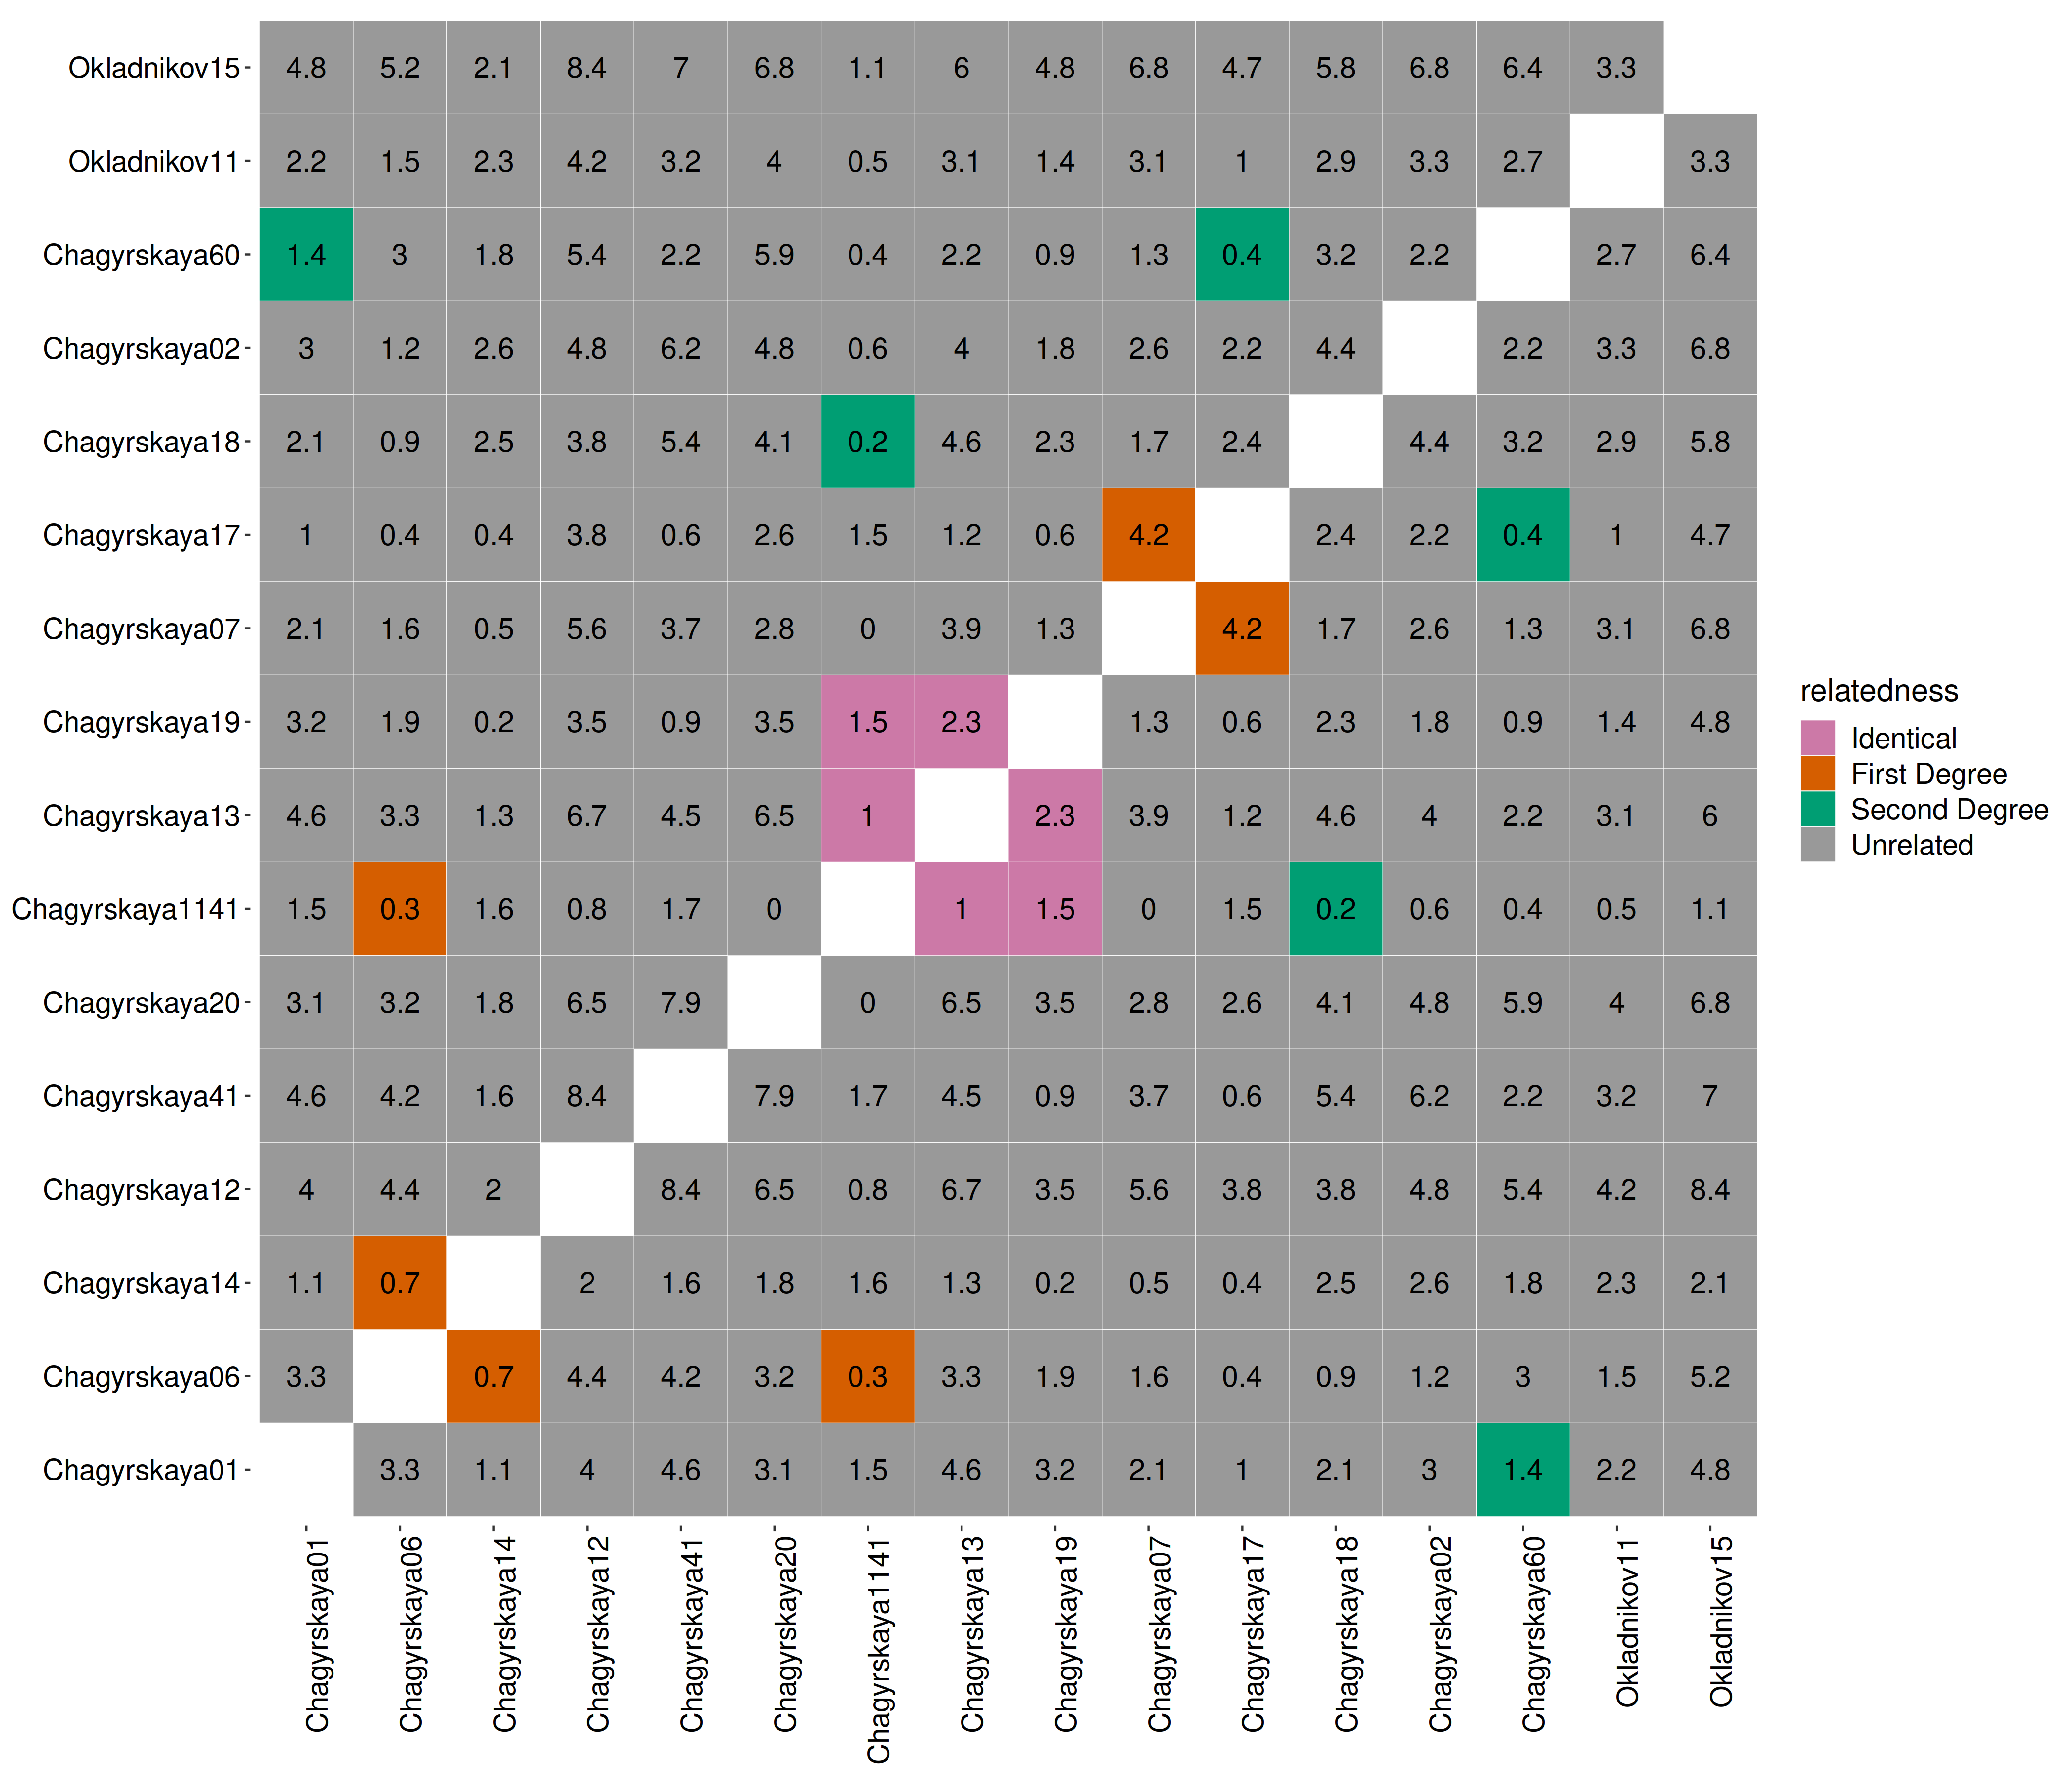
\includegraphics[width=18cm]{supplementary_info/plots/fil0_read_plot.png}
    \centering
    \caption{Application of READ on Neandertal specimens from Chagyrskaya cave. Color of a square represents the relatedness, while the number denotes standard deviations away from the upper threshold (we show lower threshold for unrelated pairs since upper threshold is not available).}
    \label{figS2:Chagyrskaya_READ}
\end{figure}


\begin{figure}[h!]
    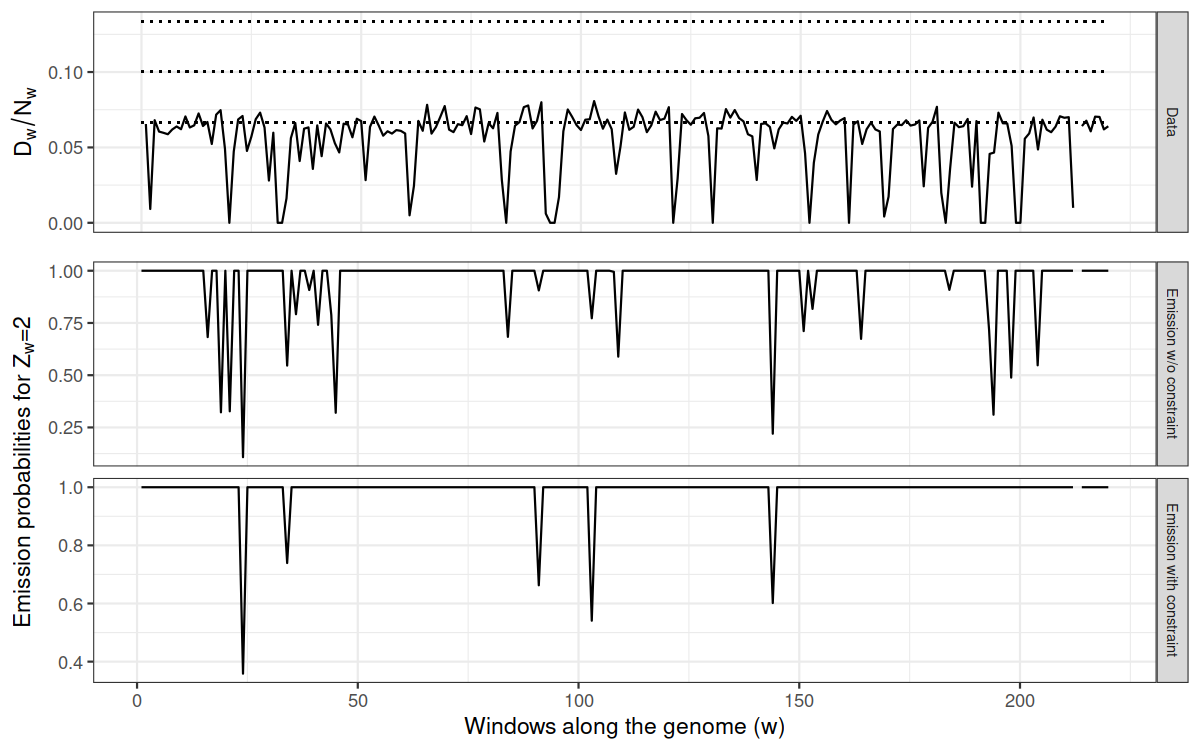
\includegraphics[width=18cm]{supplementary_info/plots/contam0_inbred1_run57_coverage0.2_asc0_inputMode_hapProbs_fil0_pair0_15_relid_emissions_bnds.png}
    \centering
    \caption{Application of identical relatedness HMM on a pair of identical individuals with low coverage (0.2x), and ROH tracts. Top panel shows pairwise proportion of differences is close to expectation, but dips in some windows due to presence of ROH tracts. Bottom two panels show $P(Data|Z=2)$ without constraints and with constraints respectively.}
    \label{figS3:bnds}
\end{figure}



\begin{figure}[h!]
    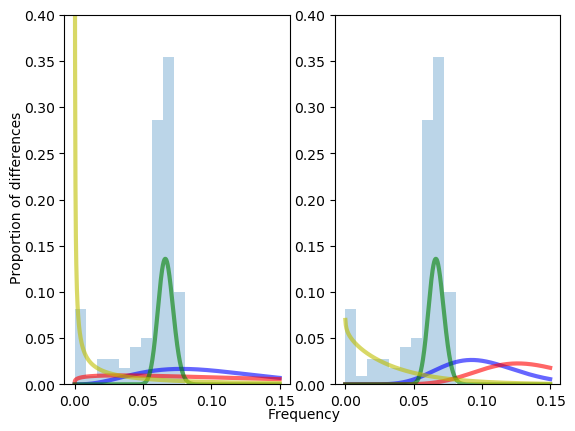
\includegraphics[width=18cm]{supplementary_info/plots/contam0_inbred1_run57_coverage0.2_asc0_inputMode_hapProbs_fil0_pair0_15_relid_betaplot.png}
    \centering
    \caption{Comparison of beta distributions estimated with the HMM (left) without and (right) with variance constraints.}
    \label{figS4:bndsbeta}
\end{figure}


\begin{figure}[h!]
    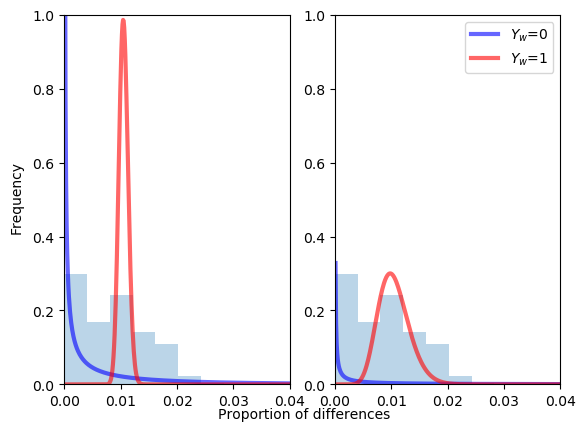
\includegraphics[width=18cm]{supplementary_info/plots/contam0_inbred1_run57_coverage0.2_asc0_inputMode_hapProbs_fil0_ind0_forced_roh.png}
     \centering
    \caption{Comparison of Beta distributions (left) without and (right) with modified emissions}
    \label{figS5:ROHforced}
\end{figure}

*Remember to use updated lcMLKIN in the plot.
\begin{figure}[h!]
    \centering
    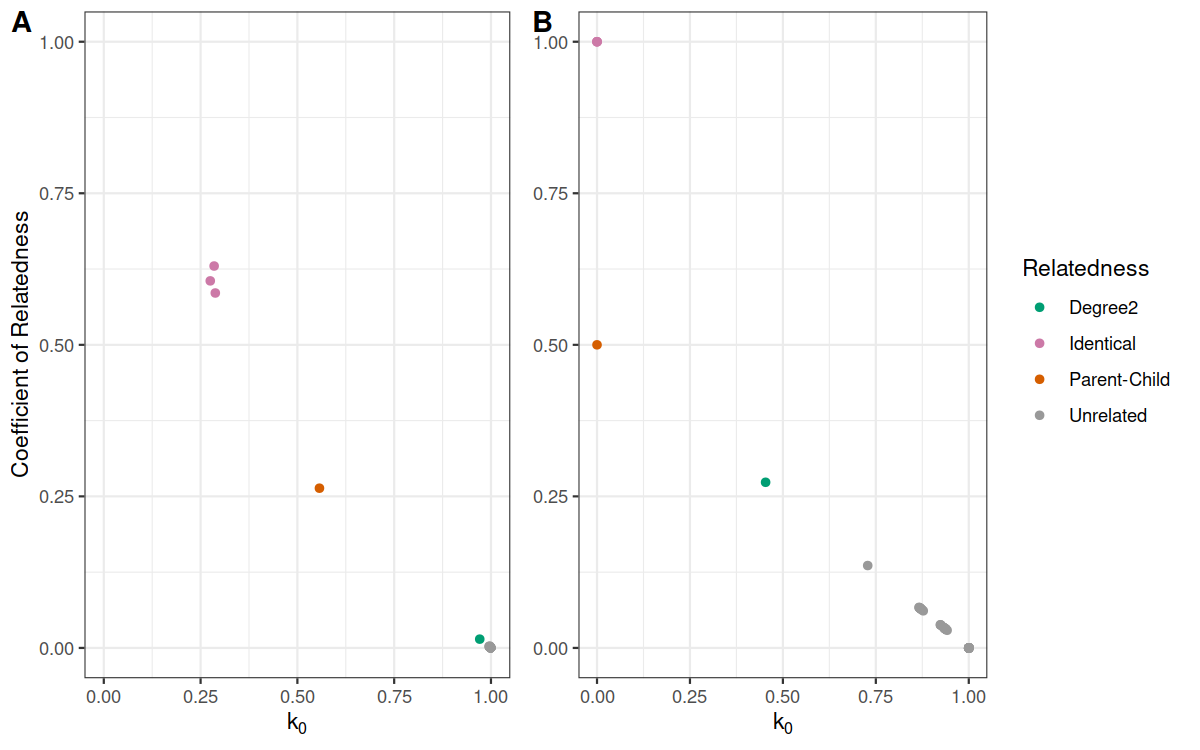
\includegraphics[width=18cm]{supplementary_info/plots/lcPlot.png}
    \caption{Comparison of IBD states estimated for Chagyrskaya specimens using (A) lcMLKIN and (B) KIN.
    The relatedness shown with different colors is estimated with and matched with READ and KIN.}
    \label{figS6:Chagyrskaya_ibd}
\end{figure}


\begin{figure}[h!]
    \centering
    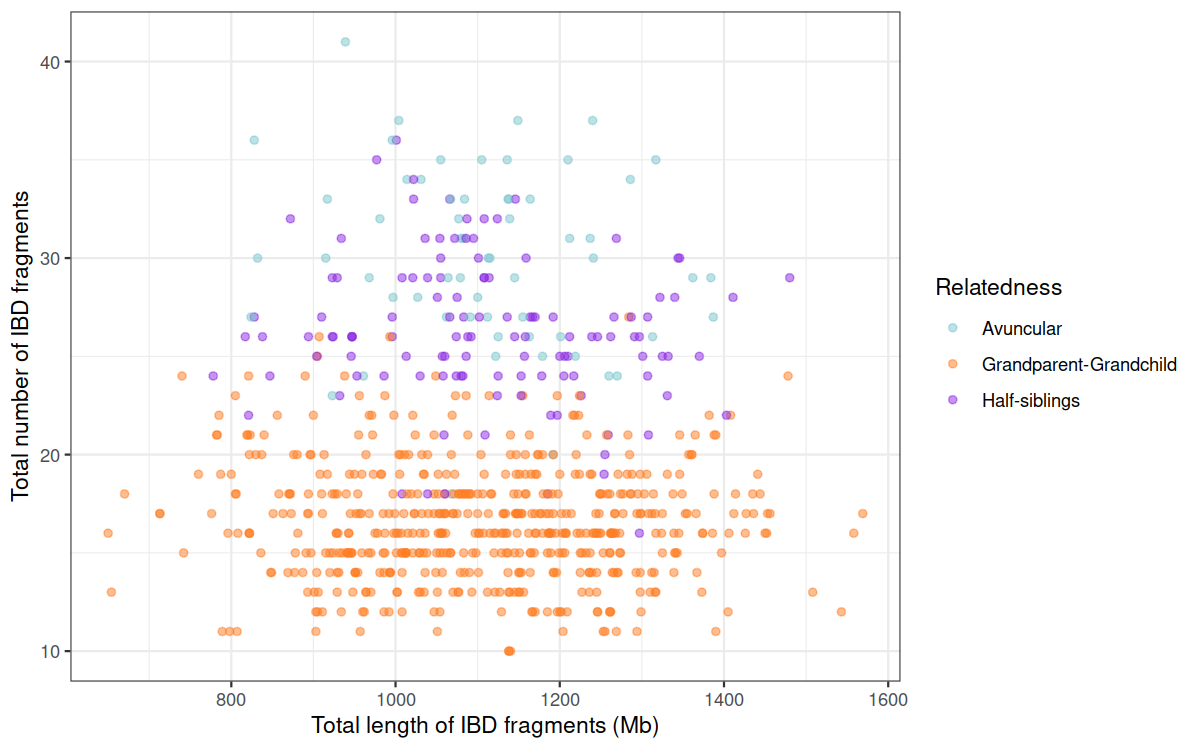
\includegraphics[width=18cm]{supplementary_info/plots/degree2_10Mwin.png}
    \caption{Avuncular and Grandparent-grandchild form different clusters, when total number of IBD fragments are plotted against total length of IBD fragments.}
    \label{figS7:second_degree}
\end{figure}


\begin{figure}[!ht]
    \centering
    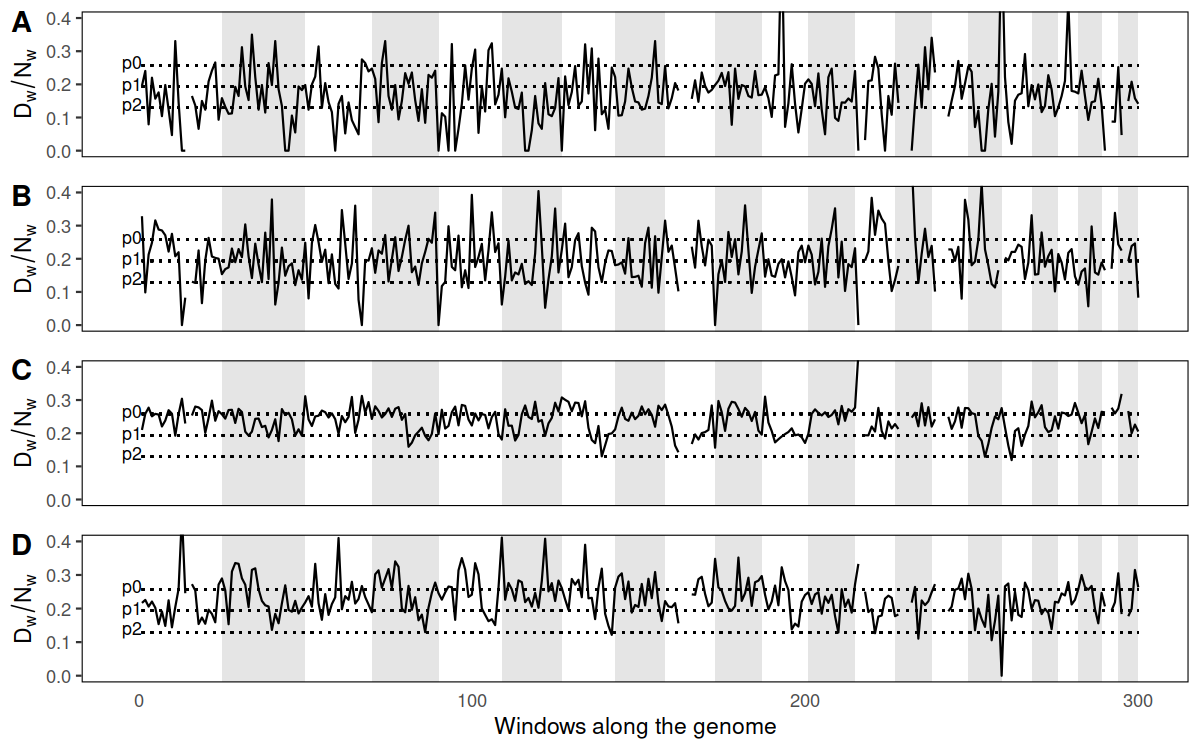
\includegraphics[width=18cm]{supplementary_info/plots/egplot1.png}
    \caption{Plots showing proportion of differences in windows along the genome for some of the pairs of relatives for which KIN differs from READ. (A) AITI62B-OTTM156 (READ estimates Identical individuals, lcMLKIN does not have sufficient data, and KIN predicts parent-child. (B) UNTA5867-UNTA5868Sk1 (READ estimates Second Degree, lcMLKIN does not have sufficient data, and KIN predicts parent-child). (C) AITI40-AITI72 (READ estimates Unrelated individuals, lcMLKIN shows 3rd-5th degree, and KIN predicts 3rd degree.)
    (D) AITI2-AITI55 (READ estimates Unrelated individuals, lcMLKIN and KIN predicts predict second degree.)}
    \label{figS8:eg1}
\end{figure}

\begin{figure}[h]
    \centering
    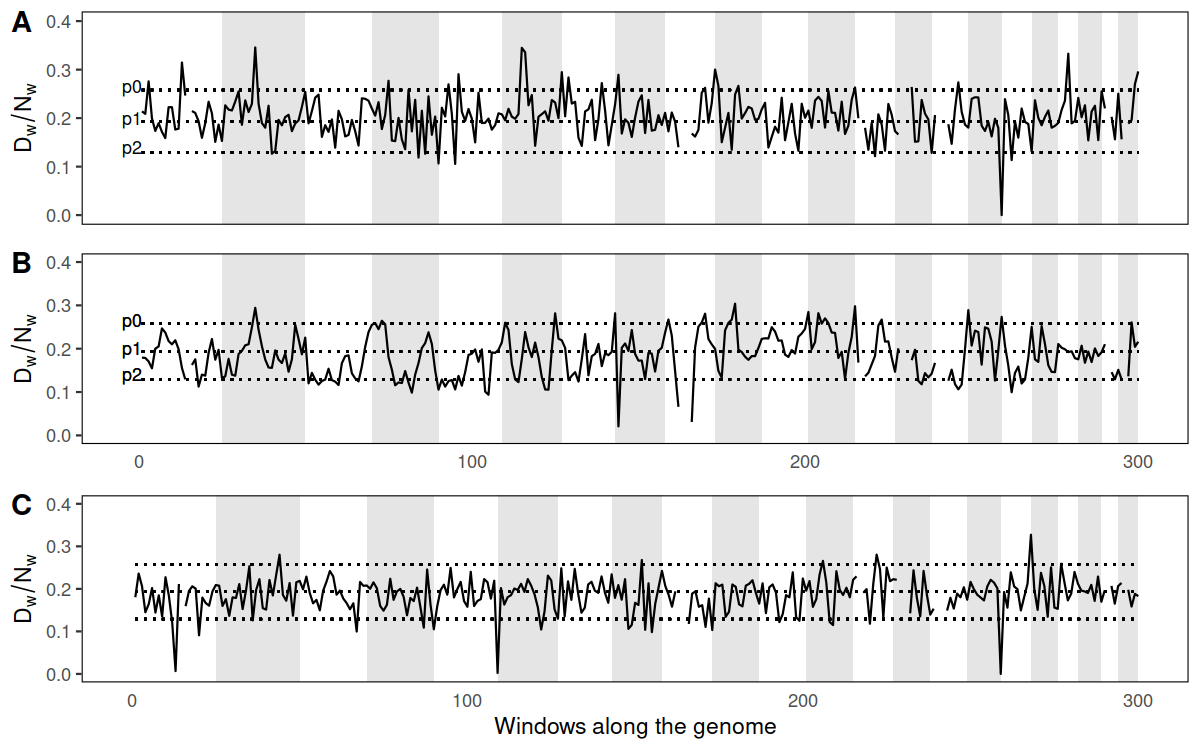
\includegraphics[width=18cm]{supplementary_info/plots/egplot2.png}
    \caption{Plots showing proportion of differences in windows along the genome for some of the pairs of relatives for which KIN differs from lcMLKIN. (A) AITI43-AITI55 (READ estimates First degree, lcMLKIN predicts siblings, while KIN predicts parent-child. (B) AITI70-AITI72 (READ estimates First degree, lcMLKIN predicts parent-child, while KIN predicts siblings.}
    \label{figS9:eg2}
\end{figure}

\bibliographystyle{plain}
\bibliography{references.bib}



\section{Notation summary}
Notation used in the paper:

\begin{itemize}
\item L: Total number of windows
\item w: Index of window
\item $N_w$: Number of sites in w
\item $D_{w}$: Number of pairwise differences in w
\item $Z_w$: Hidden IBD state in window w
\item $i$: States that $Z_w$ can take 
\item $H_w$: ROH state in window w
\item $\omega$ States that $H_w$ can take
\item A: Transition matrix
\item $\pi$: Vector of initial transition probabilities
\item $\theta$: Vector of $\pi$, A, $N_w$ for relatedness HMM
\item $p(Z_w,H_w)$: Expected proportion of differences for given $Z_w$ and $H_w$
\item $x$: Combinations of $i$ and $\omega$ states with unique $p$
\item $\delta$: Over-dispersion parameter
\item $\gamma_{wi}$: posterior probability of $H_w$
\item $h_{\omega w}$: ROH state-probabilities
\item $k_{wx}$: Posterior probability of $x$ in $w$
\item $t$: Threshold on variance of Beta distribution
\item $X$: Random variable from a beta distribution
\item $y$: Hidden homozygosity states for ROH HMM
\item $Y_w$: Homozygosity state in $w$
\item $\Theta$: Vector of $\pi$, A, $N_w$ for ROH HMM
\item $\Delta_w$: Number of differences within a library 
\item $\rho$: Expected proportion of differences in a library
\item $Gamma$: Posterior probabilities of ROH
\item $\eta$: Over-dispersion parameter used in ROH HMM
\item $\mathcal{C}$: Cost function
\item $C_l$: Contamination in library l

\item $c$: Contamination estimate for a library
\item $p_c$: Average proportion of differences between endogenous and contaminating reads
\item $p_e$:Average proportion of differences between endogenous reads
\item $p_a$: Average observed proportion of differences
\item $D_{cor,w}$: Contamination corrected number of differences in $w$
\item $N_{cor,w}$: Contamination corrected number of overlapping sites in $w$
\item $\Xi$: Endogenous read
\item $S_{cor,w}$ $N_{cor,w}$ - $D_{cor,w}$
\item $/mathbf{D_cor}$ Vector of $D_{cor,w}$
\item $G$: Genotype (0,0.5,1)
\item $\lambda$: Expected rate following Poisson distribution
\item $\nu$: Population allele frequency
\item $Lambda$: Log likelihood ratio
\item E: Expectation
\item P: Probability
\end{itemize}



\section{extra}

log lik:
\begin{align}\label{eq:1}
\log P(\BD|\theta) &= \log \sum_{\BZ} [\sum_{\BH} P(\BD|\BZ,\BH, \theta) P(\BH |\theta)] P(\BZ |\theta) \nonumber\\
&= \log \sum_{\BZ} [\sum_{\BH} \prod_w P(\BD|\BZ,\BH, \theta) P(\BH |\theta)] P(\BZ |\theta)
\end{align}


Many methods exist to estimate relatedness. Most of these work with high coverage, phased data, reference panel, population allele frequency. Other methods that work with low coverage ancient data use likelihoods, but still require 2x coverage.
methods that require a lot of things: PLINK, SNPduo,ERSA,KING,REAP,GRAB,

methods that require low coverage: SEEKIN

mtDNA and Y in relatedness READ paper[15,16,25,16]
snp data better than str when there is damage, low data
excluding related individuals, haak indo europian

READ is a very popular software to estimate relatedness in low coverage ancient DNA. It calculates distance between a pair of individuals using pseudo haploid sequences. These pairwise differences are then normalized by the median of pairwise differences in the population, and compared to the expected pairwise difference given a degree of relatedness. Expected pairwise difference for each case of relatedness is calculated using identity by descent (IBD) probabilities. 

lcMLKIN is another widely used method that uses genotype likelihoods to estimate the number of positions at which a pair of individuals have 0/1/2 chromosomes in IBD.  

REAP is a software to estimate relatedness coefficient and IBD probabilities in admixed populations, accounting for structure. It requires the number of ancestral populations, and a representation of sub population allele frequencies. 

Likelihood estimators:
Milligan BG (2003) Maximum-likelihood estimation of relatedness. Genetics
Anderson AD, Weir BS (2007) A maximum-likelihood method for the estimation of pairwise relatedness in structured populations. Genetics
Choi Y, Wijsman EM, Weir BS (2009) Case-control association testing in the presence of unknown relationships

There are various ways to measure the coefficient of relatedness r. Most methods use the probabilities of IBD to calculate r. There can be, in total 9 modes of identity described by Jacquard (1974), including the cases for 3 IBD probabilities and 3 cases of IBD. Methods assuming outbred population use only the three modes accounting for IBD. Most methods used maximum likelihood approach to estimate r (). Other methods are moment estimators that assume Hardy-Weinberg equilibrium in the population (KING, GCTA).

Discussion

Our contamination correction model requires an estimate of divergence between the contaminating and the target populations. We provide the users an option to provide a file with average pairwise difference between the two populations, or to provide a vcf file with an individual from each population. 
Pipeline has p(diff) instead of pseudohap
Methods
$$\sum_{w} \sum_{I}\sum_\omega \log P(D_{w}|Z_w, H_w)k_{w\omega i}$$



$$P(D_w | N_w, Z_w) = \sum_{k=0}^4 
\underbrace{P(D_w | N_w, k)}_{Betabinomial}
\underbrace{P(k | Z_w, H_w)}_{p matrix}
\underbrace{P(H_w =h)}_{\mathbf{h}_w}
$$

Emission probability in a window depends on both IBD state and ROH state. We obtain posterior probability of one or both individuals being ROH in each window from another HMM described in section 3.2. We calculate the cost function with beta-binomial likelihood in log space for the entire genome as:

The model can be summarised as:

\begin{equation}\label{eq:6}
P(D_w|Z_w,H_w) \sim {\sf Binom}(D_w, N_w, p_{Z,H,w})
\end{equation}

\begin{equation}\label{eq:7}
p_{Z,H,w} \sim {\sf Beta}(\alpha_{Z,H}, \beta_{Z,H})
\end{equation}

Emission probability in a window depends on both IBD state and ROH state. We calculate a cost function as the beta-binomial log-likelihood weighted by the posterior probability represented by $\gamma$.
likelihood:
\begin{align}
P(\mathbf{D},\BZ, H|\theta) &= P(\mathbf{D}|\mathbf{Z},H,\theta) P(H |\theta) P(\BZ|\theta)\nonumber\\
&= \prod_{w}  P(D_w|Z_w,  H_w, \theta) \prod_w P(H_w | \theta) \prod_{w} P(Z_w|Z_{w-1}, \theta)] P(Z_0| \theta) 
\end{align}

cost function:
\begin{equation}
    \mathcal{C} = 
       \sum_{w} \sum_{i} \log P(D_{w}|Z_w, H_w)\gamma_{wi}=
    \sum_{w} \sum_{i} 
    \log \left[\sum_{\omega}P(D_{w}|\psi_{i\omega},\delta_{i\omega}) \right] \gamma_{wi}
\end{equation}

Supplementary info:
Pipeline of KIN
Beta binomial distribution is a better fit compared to Binomial distribution for proportion of differences in windows.
Results from KIN agree with results from READ, and provide some more information about siblings/parent-child, and $3^{rd}$ Degree relatedness. 
Constraining variance of beta distributions in case of an identical pair, when identical relatedness hmm is applied, gives more accurate emission probabilities.
In figS4, the emissions improve in accuracy with constraints on variance of beta distributions. figS5 shows why we see this improvement. With variance constraints, beta distributions corresponding to Z=1 and Z=2 do not overfit the data, and higher emission probabilities seen in (A) at $D_w/N_w$=0.05 disappear. All probability distributions are scaled by the same factor so they are visible with the data histogram.
Restricting the emission probabilities at 1 for Y=1, in windows that have higher than $p_0$ difference improves the estimated Beta parameters. 
This figure shows that it is possible to differentiate between Avuncular and Grandparent-Grandchild pairs.
However, differentiating between Half-siblings may not be possible with our approach. 
*Add 1M windows result
-READ and KIN differ

-supplementary table2

\end{document}

